% Introduction
%	- Motivation
%	- RQs
%	- Contributions
%	- Outline
\chapter{Introduction}

% \section{Introduction} \label{sec:introduction}




\section{Motivation} \label{sec:motivation}

%%%
%
% Outline:
% - Current standard: terrestrial networking technology
%	- [Add papers on wired networking technology - glass fiber]
%	- Standard communication infrastructure works via cable.
%	- problem: expensive infrastructure, country borders, prone to risk [Paper] --> easy to attack wiring
%	- idea: solve most of these problems by putting up satellites which take over communication
%	- depending on height of satellite, it covers a big part of the earth's population
%	- with an antenna only, one could receive and transmit messages easily
% - Good idea, and governments already put up their networked satellite systems in order to have a fallback
%   in case some disaster appears.
%	- but not intended for the broad population
%	- intended for emergencies where little people use the system
% - in recent times, also businesses tried to use this idea and put their system up in the space, e.g,. HughesNet, ViaSat and Starlink
%	- but little is known, how well that actually works
%	- it was found that the height of satellites is the first influence
%		- GEO Satellites: Satellites at very high altitude
%		- LEO Satellites: Satellites at very low altitude
%	- Usually, GEO Satellites have a very high latency and cannot compete with LEO systems
%		- [Papers with Numbers for GEO and LEO]
%		- [Add papers that measure Starlink]
%	- However, little research is available to state clearly the performance and resilience of networked satellite systems
%		- therefore, the thesis proposed here wants to determine the current state of several networked satellite systems
%		- puts special remark on Starlink, as RIPE has many probes available for that in their measurement network
%
%%%

The internet plays a major role in our everyday's life. There are many technologies available that allow to connect to the web addressing different use cases (e.g., Wi-Fi for local area networks \cite{Henry2002} or \ac{FTTH} for high-speed wired connections to an end user's home \cite{Aleksic2010}).
However, there are several problems with such a setup. First, it requires wired infrastructure, which is quite expensive for networks in the wider area. For single end users, that is not affordable. Second, should the wired infrastructure be in place, it is vulnerable to attacks or natural catastrophes that render the service unusable.

Another emerging technology uses satellites as data transmission node. It is very resilient to human attacks or natural catastrophes as satellites are largely inaccessible. Therefore, governments installed dedicated satellite constellations to maintain communication in any given scenario. A satellite constellation is a group of artificial satellites that serve a specific purpose. Prominent examples of governmental satellite constellations are \textit{Beidou} and \textit{Galileo}.

Aside from crisis intervention, also businesses discovered opportunities. Providing communication over satellite allows users mobile access to information that usually require complex infrastructure. Users can access services like geographical data, radio frequencies, and even web access. Especially the demand for web access is growing, while companies failed at providing acceptable latencies in the past.

\begin{figure}
	\label{fig:satellitegrowth}
	\centering
	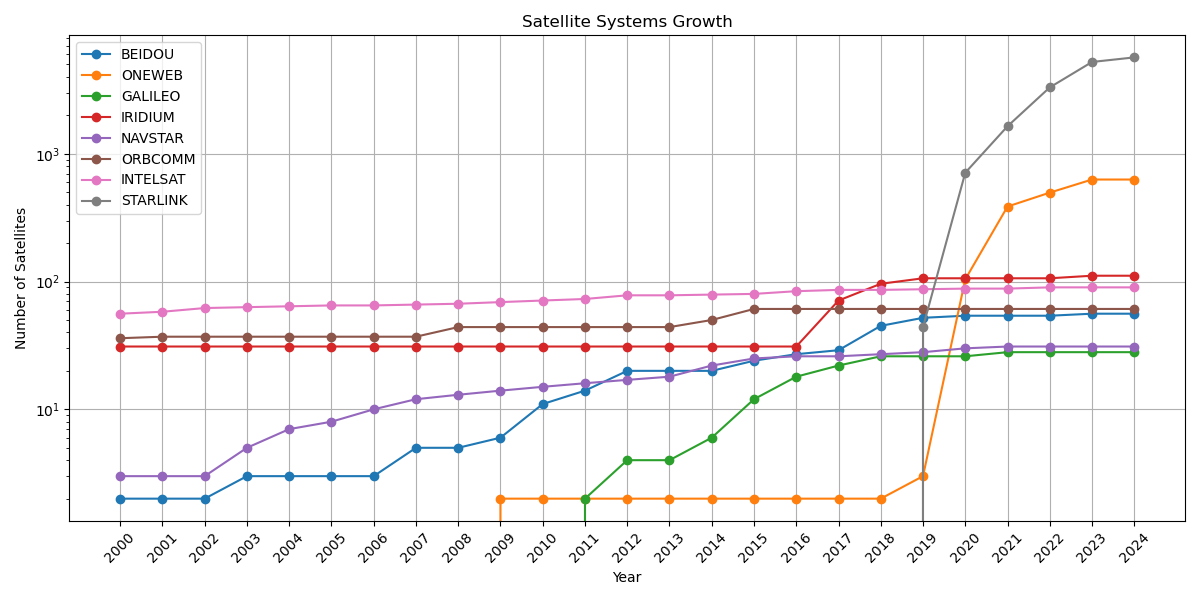
\includegraphics[width=\textwidth]{./chapters/img/satellite-growth.png}
	\caption{Growth of satellite numbers of different satellite constellations since 2000.}
\end{figure}

Therefore, different satellite communication providers (e.g., \textit{Starlink} or \textit{OneWeb}) started constructing their own networked satellite systems.
For different satellite constellations, the development of satellite numbers is shown in Figure~\ref{fig:satellitegrowth}. The numbers originate from N2YO \cite{N2YO2024}, a platform for tracking satellites.

Aside from many previous business failures \cite{Chan2002, Barboza2000}, it is still in question how well networked satellite systems actually work. Previous work reported competitive latencies for \ac{LEO} systems, but increased packet loss \cite{DBLP:conf/imc/MichelTGB22}.
Also, it is in question if networked satellite systems integrate well with existing protocols.



\section{Research Questions} \label{sec:research-questions}

\begin{mdframed}
	\textbf{RQ: How do networked satellite systems perform in terms of latency and packet loss?}
\end{mdframed}

Previous work \cite{DBLP:conf/imc/MichelTGB22, DBLP:conf/infocom/MaCZCML23, Segan2020} showed first results for \ac{RTT} (i.e., latency), throughput, and packet loss. However, networked satellite systems are a cutting edge technology that undergo changes frequently. For example, \cite{DBLP:journals/corr/abs-2403-13497}~et~al. showed a heavily different performance for moving vehicles.
Therefore, it is worth taking a look if significant changes occurred. First, we will have a look on the current performance of networked satellite systems regarding latency and packet loss. Eventually, a system displaying current Starlink performance trends could be developed.

Additionally, we will analyze the Starlink user terminal firmware to evaluate resilience and privacy of the system.

\begin{mdframed}
	\textbf{RQ: How do networked satellite systems perform efficient routing?}
\end{mdframed}

In theory, satellites should integrate well in the existing internet architecture. However, it proved not to be the case. Especially high packet loss \cite{DBLP:conf/infocom/MaCZCML23} poses a problem as a continuous connection cannot be guaranteed.
It should be determined how networked satellite systems currently route packets. That includes considering bent~pipes and ISLs \cite{Hauri2020}.

Ideally, the firmware also allows assessing whether Starlink guarantees privacy and safe data transfer to modern standard of security.
Also, we will explore the limitations of fulfilling the previously mentioned standards in networked satellite systems including \ac{ISLs} and bent pipes.

\begin{mdframed}
	\textbf{RQ: What does the Starlink user terminal firmware reveal about the system's resiliency and privacy?}
\end{mdframed}

The user terminal firmware is a key factor for privacy and resiliency of the Starlink networked satellite system.
Previous attempts in accessing the terminal's built-in firmware were highly successful, but the firmware was not analyzed in detail.

This thesis wants to explore that topic by describing a way to acquire the firmware, describe its structure, and analyze it in regard to resiliency and privacy.




% Background
%	- Networked Satellite Systems
%	- Starlink
%	- Routing: ISLs & Bent-Pipes
\chapter{Background}

\section{Satellite Communication Explained} \label{sec:satellite-communication-explained}

A satellite communication system has the target to send packets from a sender,
connected via a \ac{SNO}, to a receiver connected to a terrestrial ISP.

\begin{figure}[!ht]
	\centering
	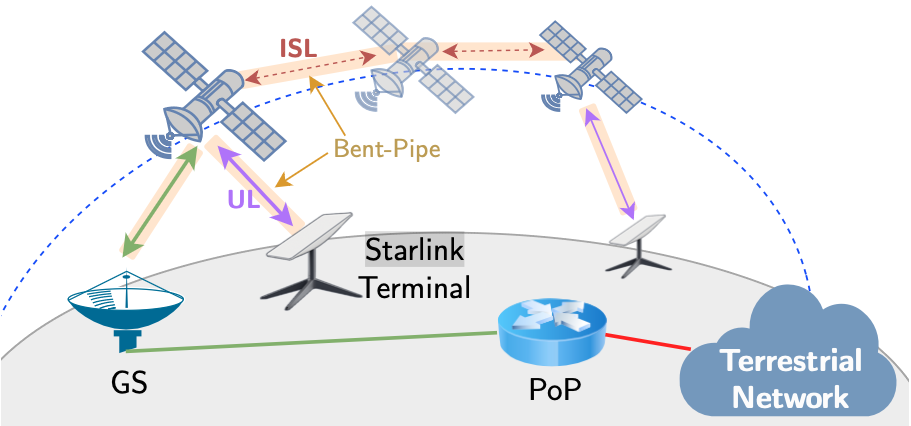
\includegraphics[width=0.7\textwidth]{./chapters/2-background/img/satcom-structure-mohan.png}
	\caption{Schematics of Satellite Communication \cite{DBLP:conf/www/MohanFCBRMO24}.}
	\label{fig:sat-com-explained}
\end{figure}

The structure is illustrated in \Cref{fig:sat-com-explained}. Initially, there
is a sender connected to a satellite antenna provided by the specific \ac{SNO}.
The satellite antenna is also colloquially called "dishy". From the senders'
perspective, there is no different use compared to a traditional terrestrial
internet connection. The antenna sends packets to a satellite that might either
forward the packets to another satellite or directly send them to a nearby
\ac{GS} (also called \ac{PoP}). The \ac{GS} serves as an "entry point" to the
terrestrial internet. A \ac{GS} can forward packets through wired connections,
so they will reach the receiver eventually. \ac{GS}s have to be provided by the
\ac{SNO}. It is essential to have a dense \ac{GS} infrastructure. Fewer
\ac{GS}s can induce higher latencies, as more hops might be necessary.
Therefore, it is necessary to determine an advantageous positioning of \ac{GS}s
\cite{DBLP:conf/sigcomm/VasishtSC21}. For reference, one can get an overview of
current placements of Starlink and OneWeb \ac{GS}s on
\url{https://satellitemap.space}.

The technology of communicating with satellites will not be explained here.
Amongst others, it is described by Pratt~et~al.~\cite{pratt2019satellite}.

Theoretically, the propagation of data in satellite communication happens at
the speed of light. However, the latencies still vary a lot depending on the
choice of \ac{SNO}. Each of them provides a different satellite constellation.
One of the dominating factors is the altitude of the satellites in the
constellation. The higher the satellites are positioned, the more region a
single satellite covers. Therefore, fewer satellites are required to cover a
specific region, which reduces costs. Usually, \ac{SNO}s structure the earth's
surface in cells that receive coverage by at least one satellite. In the case
of Starlink, the world is divided in cells in the form of a hexagon with a
diameter of $\approx 24.13~km$. That translates to a single satellite being
able to cover approximately $379~km^2$ \cite{Pekhterev2021}.

Overall, one differentiates between \ac{GEO} (35'786 km altitude), \ac{MEO}
(2'000 - 35'786 km altitude), and \ac{LEO} (< 2'000 km altitude) satellite
constellations. One can see in \Cref{eq:geo-min-latency} and
\Cref{eq:starlink-min-latency} that this has a significant impact on the
latency.

\begin{equation}
	\frac{2 \cdot 35'786 km}{300'000 \frac{km}{s}} \approx 0.240 s
	\label{eq:geo-min-latency}
\end{equation}
\begin{equation}
	\frac{2 \cdot 550 km}{300'000 \frac{km}{s}} \approx 0.004 s
	\label{eq:starlink-min-latency}
\end{equation}

A \ac{GEO} constellation has a minimum latency of around 240 ms, as shown in
\Cref{eq:geo-min-latency}, assuming a packet needs to reach a satellite in
\ac{GEO} altitude and get back to the earth's surface. On the other hand,
\Cref{eq:starlink-min-latency} shows that a \ac{LEO} satellite constellation at
an altitude of 550 km (like in the case of Starlink) has a minimum latency of
only 4 ms. Research has shown that also in practice \ac{LEO} constellations are
superior compared to \ac{GEO} constellations, especially in terms of latency
\cite{DBLP:journals/pacmnet/RamanVCSZ23, Segan2020}. However, terrestrial
internet still performed better compared to \ac{LEO} constellations
\cite{DBLP:conf/www/MohanFCBRMO24, DBLP:conf/infocom/MaCZCML23}.

\subsection{Bent-Pipes} \label{sec:bent-pipes}

Ground stations are required for satellites to route packets to a receiver.
Depending on the location of the sender, the first satellite on the route might
have to forward packets to a different satellite (using an \ac{ISL}) in order
to reach a region with a \ac{GS}. Such a route is called "Bent-Pipe". Depending
on the number of hops in-between satellites, it is called an "n-hop-bent-pipe".
If the packet needs to be forwarded only once, it is a 1-hop-bent-pipe.

It is in question how bent-pipes influences the performance and behavior of a
networked satellite system. Research still discusses whether bent-pipes provide
a positive (\cite{DBLP:conf/hotnets/HauriBGS20}) or negative
(\cite{DBLP:conf/www/MohanFCBRMO24}) impact.


\section{Use Case of Networked Satellite Systems} \label{sec:usecase-networked-satellite-systems}

The internet has become a key-technology for communication in nearly every
aspect of the society. Having no access to the internet will result in
significant drawbacks. However, internet requires a complex infrastructure with
high cost. Especially in distant location with little population, building such
an infrastructure will not be affordable.

Therefore, people came up with the idea of using satellites to communicate with
distant locations. In theory, only three satellites are required to communicate
with any point on earth (except for polar regions)
\cite{DBLP:conf/5gwf/HofmannK19}. The cost of providing this number of
satellites is much less compared to the costs of providing a terrestrial
network infrastructure with similar accessibility.

There is a group of people that will likely never receive terrestrial network
infrastructure: people on boats and planes. While there is cellular internet
access, it is not offered on the sea and in the high sky. Therefore, the only
option of internet access is satellite internet, which is served all over the
world.

Additionally, networked satellite systems are much more resilient to physical
influences like earthquakes, terrorist attacks, or storms
\cite{DBLP:conf/pam/StevensIBD24}. Terrestrial infrastructure can be destroyed
easily and therefore especially governments contracted networked satellite
system ISPs. A prominent example is the use of Starlink in conflict zones like
Ukraine.

\section{Satellite Network Operators} \label{sec>isps}

There are a couple of \ac{SNO}s out there providing internet access via
satellite network. Table~\ref{fig:satellite-isp} shows different \ac{SNO}s for
networked satellite systems.

\begin{table}[]
	\caption{Different networked satellite ISPs}
	\label{fig:satellite-isp}
	\begin{tabular}{lrr}
		\toprule
		ISP       & Category & Customer Group      \\
		\midrule
		Starlink  & LEO      & Private \& Business \\
		OneWeb    & LEO      & Business            \\
		HughesNet & GEO      & Private \& Business \\
		Intelsat  & GEO      & Business            \\
		Viasat    & GEO      & Business            \\
		Orbcomm   & GEO      & Business            \\
		Iridium   & GEO      & Private \& Business \\
		\bottomrule
	\end{tabular}
\end{table}

They differentiate mostly by providing either a \ac{LEO} or \ac{GEO} service.
The only \ac{LEO} \ac{SNO}s are Starlink and OneWeb. Starlink has an economical
advantage over most of its competitors as they are a sub-company of SpaceX.
SpaceX is a company providing spacecraft manufacturing and launch services.
This makes the launch of satellites less tedious compared to Starlink's
competitors.

Kohnmann \cite{Kohnmann24} reported about Amazon's intentions of launching a
\ac{SNO} called Kuiper. It is planned to be launched by the end of 2026, after
two test satellites were already launched
(\href{https://www.n2yo.com/satellite/?s=58014}{KUIPER-P2}, ID58013 and
\href{https://www.n2yo.com/satellite/?s=58013}{KUIPER-P1}, ID58014) on
October~6,~2023. However, there is no data yet available.

\section{Satellite Network Simulators} \label{sec:satellite_network_simulators}

Amongst concrete measurements, one can also simulate networked satellite
systems. This became increasingly interesting when the constellations were
composed of many more satellites compared to traditional \ac{GEO} satellite
constellations. For example, \ac{LEO} constellations comprise hundreds to
thousands of satellites, which implies a highly complex system.

Sadly, measurements are often highly difficult as they either require acquiring
satellite hardware or recruiting users that already posses the required
hardware. Simulation would tackle both problems, while maintaining low cost. To
the best of our knowledge, we found two networked satellite simulators for
\ac{LEO} constellations.

\subsection{StarPerf} \label{sec:starperf}

\textit{StarPerf}\footnote{\href{https://github.com/SpaceNetLab/StarPerf\_Simulator}{SpaceNetLab/StarPerf\_Simulator}}
\cite{DBLP:conf/icnp/LaiLL20} is a mega-constellation performance simulation
platform. It specifically aims at measuring the impact of the movements of
satellites. Also, it measures performance in different areas. However, setting
it up required, amongst others, Matlab and STK. This made the project difficult
and expensive to test. Therefore, we did not advance in trying out
\textit{StarPerf}.

\subsection{Hypatia} \label{sec:hypatia}

\textit{Hypatia}\footnote{\href{https://github.com/snkas/hypatia}{snkas/hypatia}}
\cite{DBLP:conf/imc/KassingBASS20} is another LEO network simulation framework,
released in 2020 just like \textit{StarPerf}. It aims at a low-level simulation
on packet-level and visualizes the data. Unlike \textit{StarPerf}, it only
requires a Python3 installation. Sadly, running simulations with Hypatia is
highly complex as it requires the user to define, amongst others, the
satellites, ground stations, and points of presence. This information is hardly
available, which renders the simulations barely usable.

\subsection{Problems of Network Simulators}

To the best of our knowledge, research has stopped relying on simulators since
2020. There is proper hardware available that allows testing in the real world.
Testing in the real world has the advantage as it takes more variables into
account. Crucial factors for the performance of a networked satellite system
are the weather, congestion, solar magnetic storms, material failure, and many
more. Those cannot be ideally tested with simulations and will eventually
produce wrong results. Therefore, for further research of this thesis,
simulations will not be used.


% Satellites
\section{Growth of Satellite Constellations} \label{sec:satellite-constellations}

Recent years saw a rapid development of satellite technology, especially due to
the growing demand of global connectivity and communication. Therefore,
companies constructed their own satellite constellations leading to a total
number of more than 29'000 objects (according to N2YO in September 2024) in
space at the time of writing.

\begin{figure}[ht]
	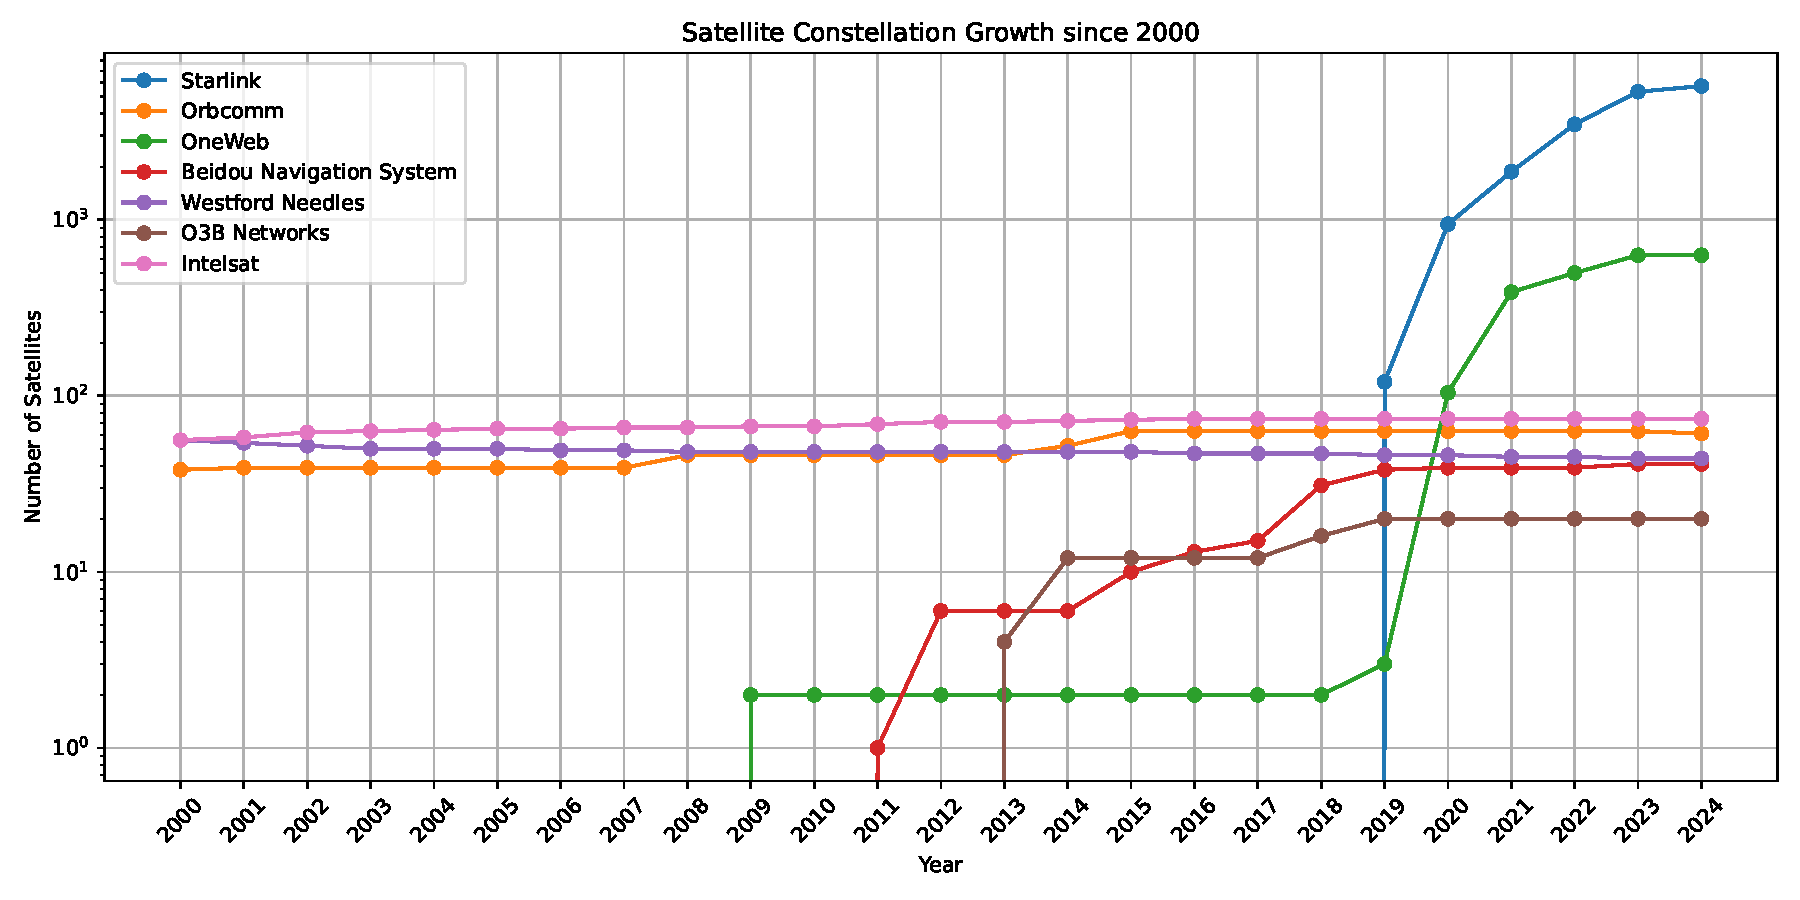
\includegraphics[width=\textwidth]{./chapters/2-background/satellites/img/satellite-dev.pdf}
	\caption{Growth of number of satellites in different satellite constellation from 2000 to 2024 (note the logarithmic scale).}
	\label{fig:growth-satellite-constellations}
\end{figure}

\begin{table}
	\caption{Growth of various satellite constellations from 2017 to 2024}
	\label{fig:satellite-constellations-short}
	\begin{tabular}{lrrrrrrrr}
		\toprule
		                          & 2017 & 2018 & 2019 & 2020 & 2021 & 2022 & 2023 & 2024 \\
		Classification            &      &      &      &      &      &      &      &      \\
		\midrule
		\textbf{Starlink}         & 0    & 0    & 120  & 943  & 1871 & 3481 & 5326 & 6396 \\
		\textbf{Orbcomm}          & 63   & 63   & 63   & 63   & 63   & 63   & 63   & 61   \\
		\textbf{OneWeb}           & 2    & 2    & 3    & 104  & 388  & 498  & 628  & 628  \\
		\textbf{Beidou}           & 15   & 31   & 38   & 39   & 39   & 39   & 41   & 41   \\
		\textbf{Westford Needles} & 47   & 47   & 46   & 46   & 45   & 45   & 44   & 44   \\
		\textbf{O3B Networks}     & 12   & 16   & 20   & 20   & 20   & 20   & 20   & 20   \\
		\textbf{Intelsat}         & 74   & 74   & 74   & 74   & 74   & 74   & 74   & 74   \\
		\bottomrule
	\end{tabular}
\end{table}


Figure~\ref{fig:growth-satellite-constellations} shows various satellite
constellations with the number of satellites it consisted of per year.
Table~\ref{fig:satellite-constellations-short} show the corresponding numbers,
starting in 2017. One can see that Starlink is by far the numerically largest
constellation. At the time of writing, it has 6'396 satellites. The Starlink
constellation grew from 2022 to 2023 by nearly 2000 satellites. OneWeb,
Starlink's closest competitor, has a total of 628 satellites with no change
between 2023 and 2024.

Other satellite communication constellations like Orbcomm or Intelsat did not
grow at all, or even lost satellites. Only Starlink and OneWeb see significant
growth in recent years. However, this is also due to the requirement of LEO
constellations (i.e., Starlink and OneWeb) of having significantly more
satellites, compared to GEO constellations (e.g., Intelsat and O3B~Networks).



% Related Work

% Methodology
%	- Data Sources
%	- Created Data Set
%	- IPInfo
\chapter{Methodology}

\section{Data Collection} \label{sec:data-collection}

For analysis, we create a dataset containing measurements from various sources
about networked satellite systems. Sadly, only data from Starlink devices was
included in the thesis as other \ac{SNO}s did not have sufficient data openly
available.

The data originates from RIPE Atlas, Cloudflare Radar, and N2YO. While
N2YO provides data about satellites, the others hold measurement results. In
the case of N2YO, the website was crawled, while the others provide API
access. The process of data collection is illustrated in
Figure~\ref{fig:data-collection-process}.

\begin{figure}[h]
	\centering
	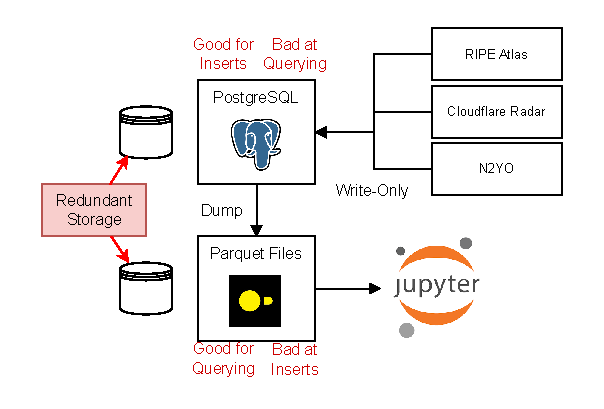
\includegraphics[width=\textwidth]{./chapters/3-methodology/img/architecture.drawio.pdf}
	\caption{Architecture of Data Collection}
	\label{fig:data-collection-process}
\end{figure}

The data is collected from each platform and inserted into a PostgreSQL
database. The database shall allow producers to quickly insert new data (i.e.,
new rows). Transactional databases are the best choice for that, e.g.,
PostgreSQL. To quickly analyze data, an analytical database is the best choice.
For that purpose, Parquet files can be used. Therefore, the data from
PostgreSQL is dumped into the Parquet files. This creates a redundant storage,
in exchange for analysis speed. The resulting data format is shown in
Figure~\ref{fig:er-diagram}.

\begin{figure}
	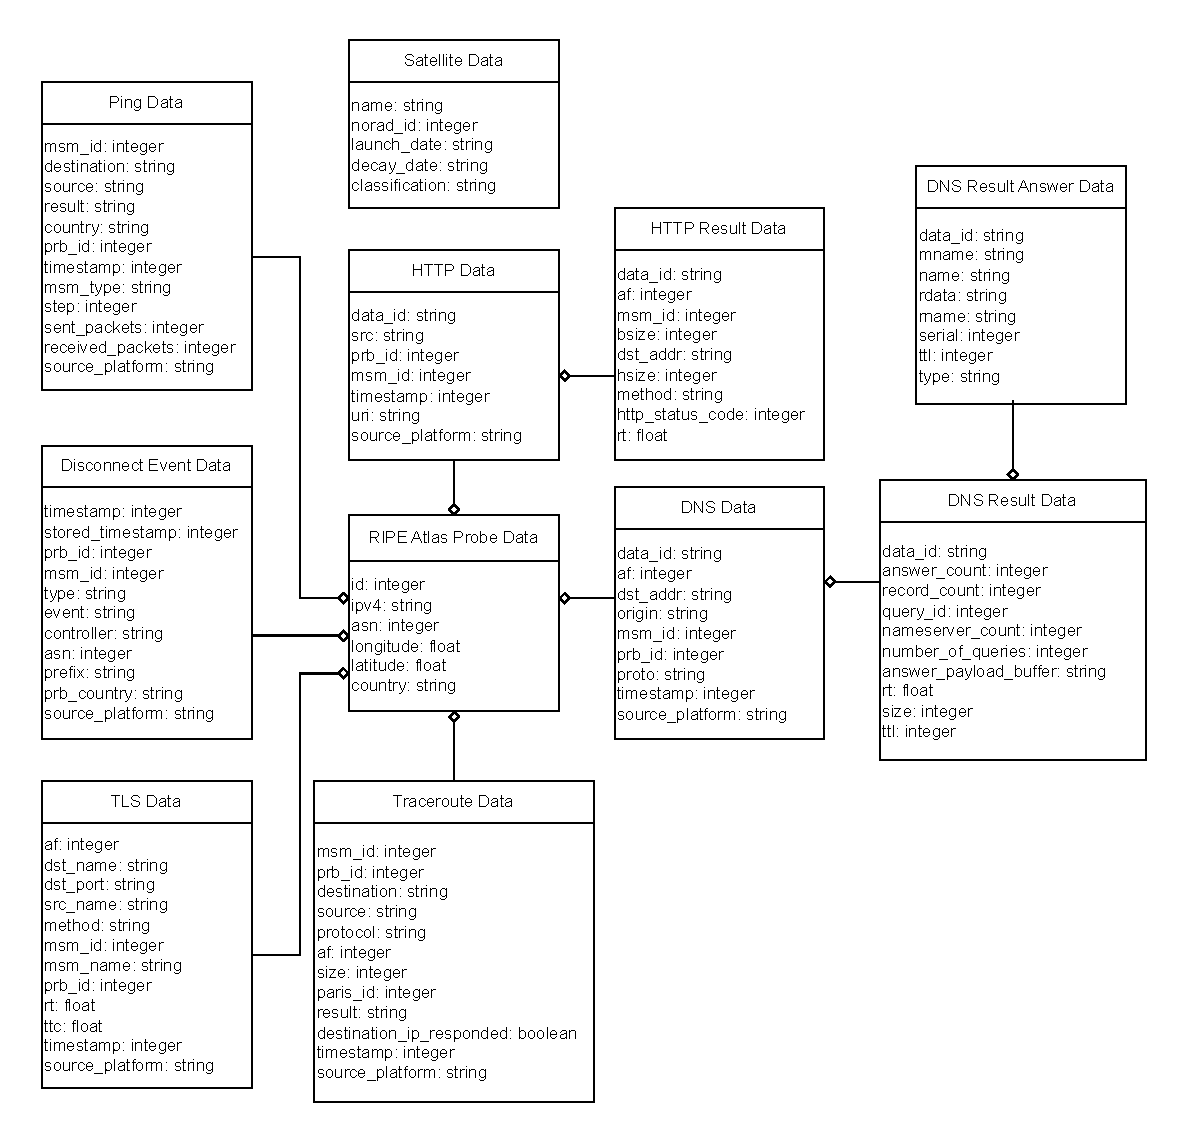
\includegraphics[width=\textwidth]{./chapters/3-methodology/img/er-diagram.drawio.pdf}
	\caption{ER Diagram of Data Schema in PostgreSQL Database.}
	\label{fig:er-diagram}
\end{figure}

The database includes Ping, Traceroute, TLS, HTTP, Disconnect Event, and DNS
measurement data, as well as information about the RIPE~Atlas probes and all
satellites ever launched (including rocket bodies). The whole database
comprises more than 150 GB in PostgreSQL ($\approx$ 50 GB in Parquet files).

Additionally, the measurement data is enriched with data from IPinfo during the
analysis process. However, this data is not included in the dataset and has to
be obtained from IPinfo itself.

\subsection*{RIPE Atlas Data}

RIPE Atlas offers various probes connected via networked satellite systems. At
the moment of writing, all of those probes are connected via Starlink.
Therefore, all the data from RIPE Atlas probes is Starlink data.

Probes are computers running the
\href{https://github.com/RIPE-NCC/ripe-atlas-software-probe}{probe software
	from RIPE Atlas}. They are centrally connected to the RIPE Atlas
servers and
can be used by any person to perform measurements against them. The possible
measurements are defined by the
\href{https://atlas.ripe.net/docs/apis/rest-api-reference/}{RIPE Atlas REST
	API}.

Overall, there are 150 probes from 26 countries. Each probe performs basic
measurements on a regular schedule (so-called built-in measurements). The
built-in measurements are the main source of data and serve as historical
record. This allows to analyze data from 2022. Even if there is Starlink data
prior to 2022, it originates from very little probes and therefore will not be
considered in this thesis to avoid unreliable data.

\section{Reproducibility of Results and Data} \label{sec:reproducibility}

The code to reproduce the results and data is uploaded to GitHub\footnote{See \url{https://github.com/starlink-thesis-diic/starlink-thesis}}. The user is only required to have a running internet connection and an installation of Nix and Docker. Follow the instructions provided by the repository to obtain the results and data by yourself\footnote{The scripts might not work, if data format in the sources has changed since the last update of the scripts.}.

\section{Measurement Platforms} \label{sec:measurement-platforms}

The following chapter describes the measurement platforms that were used to
measure and collect data.

\subsection{RIPE Atlas} \label{sec:ripe-atlas}

RIPE~Atlas is an open measurement platform to perform basic measurements on the
internet. It holds more than ten thousand probes that serve as start points. A
probe is machine that has the RIPE Atlas probe software installed. A user can
request a probe for a measurement (e.g., a ping from a probe to a RIPE NCC root
server).

RIPE Atlas offers the following basic types of measurements:

\begin{itemize}
	\item Ping
	\item Traceroute
	\item (Dis)connection Events
	\item DNS Lookup
	\item DNS TLDs
	\item HTTP
	\item TLS (SSL) GET Certificate
\end{itemize}

RIPE Atlas offers the possibility to start measurements via the web interface
or an API. While the web interface is sufficient for most use cases, it is also
quite limited. Using the API offers more possibilities (e.g., turning DoH
queries into DoTLS by adding \verb|"tls": true| into the definition of the
measurement).

Additionally, each registered probe performs measurements on a regular basis in
fixed time intervals (e.g., each probe performs every 240 seconds a ping
measurement against all RIPE NCC root servers). Those measurements are called
built-in measurements. They run always when the probe is only and connected to
the RIPE Atlas network. The built-in measurements are the ones used for the
data of this thesis within a specified time interval (usually January 2022 to
June 2024).

Downloading the results of a measurement also works by accessing the API. For
previous results, one can access the REST API that stores all results ever
measured. For more up-to-date results, one can use the Streaming API that sends
the most recent results to a subscribed socket.

Theoretically, the API is rate-limited, but we did not encounter problems even
when bulk-downloading larger datasets. Still, ethical crawling was used.

\subsection{Cloudflare Radar} \label{sec:cloudflare-radar}

Cloudflare manages a vast amount of traffic on the internet. Initially, it
served the purpose of protecting servers from attacks. Today amongst others, it
also manages traffic, and sells data. In 2020, Cloudflare released data that
has been held internal. This new platform is \ac{CFR}. \ac{CFR} offers various
statistics on the internet ranging from security statistics over latency
measurements to bot ratios per country.

For the purpose of this thesis, we are mostly interested in the performance
measurements. \ac{CFR} offers performance measurements within their \ac{IQI}.
It is the collection of measurements performed through their
\href{https://speed.cloudflare.com/}{Internet Speed Test}
\cite{DavidBelson2023, CloudflareRadarDocsIQI}. As target, \ac{CFR} uses a
fixed set of Cloudflare servers.

\begin{takeaway}{Difference of RIPE Atlas and Cloudflare Radar}
	Measurements performed in \ac{CFR} and RIPE Atlas differentiate in the
	targeted servers (root servers vs. Cloudflare servers), the measurement
	probe (RIPE Atlas probe vs. browser), and the metric used (TLS vs. Time
	to First Byte). Cloudflare's servers are expected to have a better
	latency (they claim to be ~50ms away from 95 \% of the earth's
	population; State September 17, 2024).
\end{takeaway}

\begin{figure}
	\begin{subfigure}[t]{0.48\textwidth}
		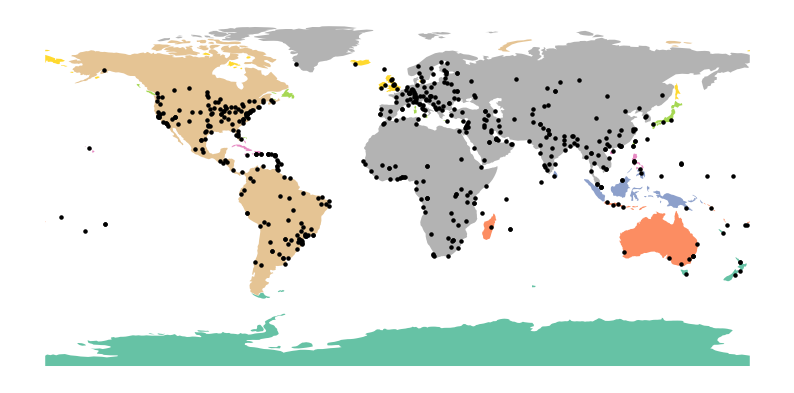
\includegraphics[width=\textwidth]{./chapters/3-methodology/img/rootserver-locations.png}
		\caption{Locations of Root Servers (all *.root-servers.org
			together) \cite{rootservers092024}}
	\end{subfigure}
	\begin{subfigure}[t]{0.48\textwidth}
		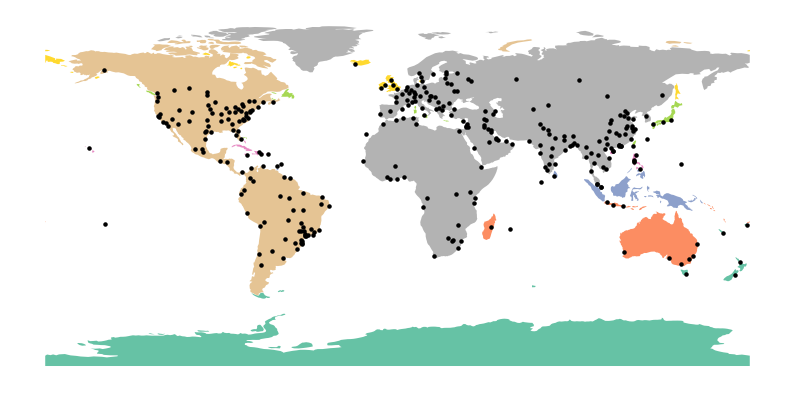
\includegraphics[width=\textwidth]{./chapters/3-methodology/img/cloudflare-datacenter-locations.png}
		\caption{Locations of Cloudflare Data Centers
			\cite{CloudflareGlobalNetwork2024}}
	\end{subfigure}
\end{figure}

% TODO: Do I actually need this?
\subsection{OONI} \label{sec:ooni}

\subsection{N2YO} \label{sec:n2yo}

N2YO is a platform collecting data about satellites in space. It is a data
integration platform collecting data from different platforms like Celestrak
and Space-Track.

For the purpose of this thesis, N2YO is used to find information on the
development of various satellite constellations. Therefore, we want to find the
following information:

\begin{itemize}
	\item Satellite ID (also formerly called Norad ID)
	\item Satellite Name
	\item Launch Date
	\item Decay Date (if applicable)
	\item Classification (if applicable)
\end{itemize}

Each satellite receives a unique ID, centrally given to all satellites
launched. It is a continuous number starting at 1. The satellite with ID~1 is
the rocket body of Sputnik~1. Sputnik~1 itself holds ID~2.

The data is obtained by a web crawler that parses the HTML page and finds the
information needed. There is also the possibility of getting the data by API,
but the API is rate-limited. Parsing HTML is inefficient, but still a quicker
approach compared to using the API.


% Results
%	- Satellite Constellations
%	- Packet Loss by Country and Month
%	- Latency by Country and Month
%	- Correlation of Packet Loss and Latency
%	- Routing with Starlink
%	- TODO(robert): What more?
\chapter{Results}

\section{Performance of Networked Satellite Systems}

%
%	Performance
%

% Latency
\subsection{Packet Loss from 2022 to 2024} \label{sec:packet-loss}

We looked at the packet loss for the time range from 2022 to June 2024. We use
the Ping measurement from the RIPE Atlas built-in measurements, which by
default send three packets and collect the number of received packets.
Table~\ref{fig:packetloss-total} shows the resulting packet losses in percent
per country.

\begin{table}
	\footnotesize
	\caption{Packet Loss and Latency Correlation in 2022 to June 2024}
	\label{fig:packetloss-total}
	\begin{tabular}{rrlr}
		\toprule
		Sent      & Received  & Country                     & Packet
		Loss Ratio in \%                                             \\
		\midrule
		2150628   & 2134905   & Austria                     & 0.73   \\
		65021654  & 62438854  & Australia                   & 3.97   \\
		22727113  & 22211676  & Belgium                     & 2.27   \\
		1176124   & 1168114   & Benin                       & 0.68   \\
		124263104 & 121160149 & Canada                      & 2.50   \\
		2843      & 2832      & Switzerland                 & 0.39   \\
		3626230   & 3617474   & Chile                       & 0.24   \\
		8092876   & 8074360   & Czechia                     & 0.23   \\
		96089885  & 85983781  & Germany                     & 10.52  \\
		21714610  & 21001677  & Spain                       & 3.28   \\
		432934    & 418925    & Falkland Islands (Malvinas) & 3.24   \\
		321919833 & 299847062 & France                      & 6.86   \\
		83840509  & 80720387  & United Kingdom              & 3.72   \\
		12522224  & 12318835  & Greece                      & 1.62   \\
		271185    & 265100    & Guam                        & 2.24   \\
		18472787  & 18217243  & Haiti                       & 1.38   \\
		37188354  & 35583136  & Italy                       & 4.32   \\
		4160290   & 3829356   & Kiribati                    & 7.95   \\
		127756    & 121937    & Madagascar                  & 4.55   \\
		20450037  & 17548642  & Netherlands                 & 14.19  \\
		26654399  & 21785387  & Philippines                 & 18.27  \\
		18739794  & 18670207  & Poland                      & 0.37   \\
		7047181   & 6967111   & Réunion                     & 1.14   \\
		9975257   & 9922734   & Sweden                      & 0.53   \\
		578852548 & 557475491 & United States               & 3.69   \\
		18571694  & 18463935  & Virgin Islands, U.S.        & 0.58   \\
		\bottomrule
	\end{tabular}
\end{table}

The results are surprising as some countries experience very high packet
losses, while other neighboring countries have rather low packet loss ratios.
For example, Germany and Netherlands are well-developed countries with a
relatively high number of \ac{GS}es. One would expect a low packet loss, which
is not the case. Both countries hold packet loss ratios above ten percent. On
the other hand, neighboring countries like Austria do not show such a pattern.
Another country with remarkably high packet loss are the Philippines, which
have the highest packet loss ratio of all countries.

Overall, most countries experience packet loss ratios at one to four percent,
with some having an even lower value. The lowest value has Czechia with
0.23~\%, while Chile has 0.24~\%.

However, the time range is quite long. Therefore, we looked at the time range
in a more fine-grained interval for the above-mentioned countries.
Figure~\ref{fig:packet-loss-fine-grained} show the packet loss ratios for each
month from January 2022 to June 2024 for Germany, the Netherlands, the
Philippines, and the USA. The first three were chosen as they are noticeable in
Table~\ref{fig:packetloss-total}. The USA was chosen, as it holds the most data
and is therefore a good comparison.

\begin{figure}
	\centering
	\begin{subfigure}[t]{0.47\linewidth}
		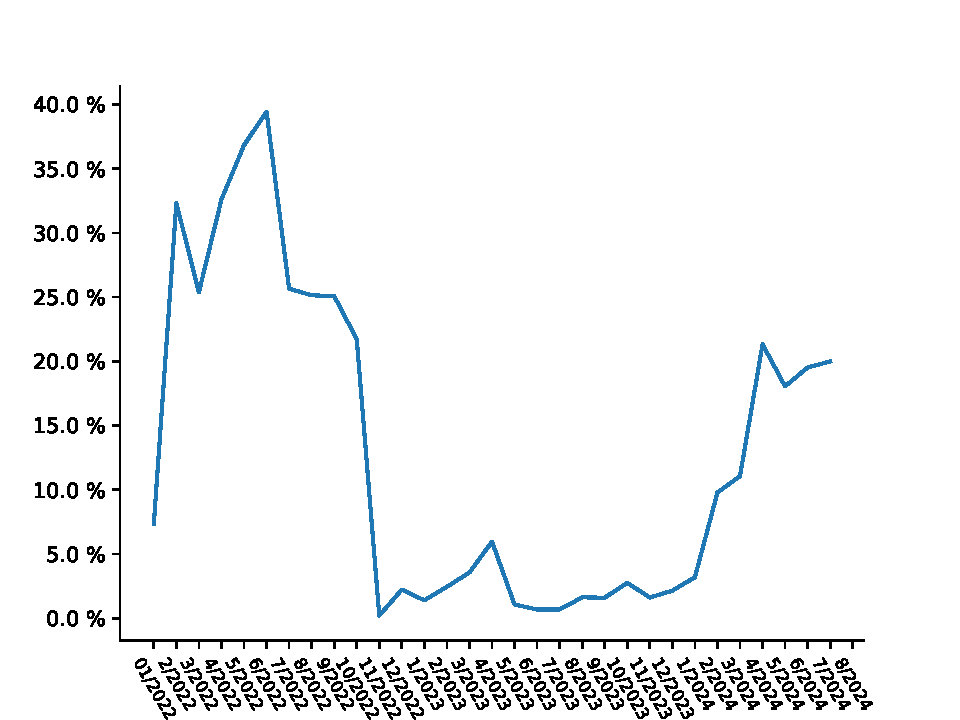
\includegraphics[width=\linewidth]{./chapters/4-results/packet-loss/img/DE.pdf}
		\caption{Germany}
	\end{subfigure}
	\begin{subfigure}[t]{0.47\linewidth}
		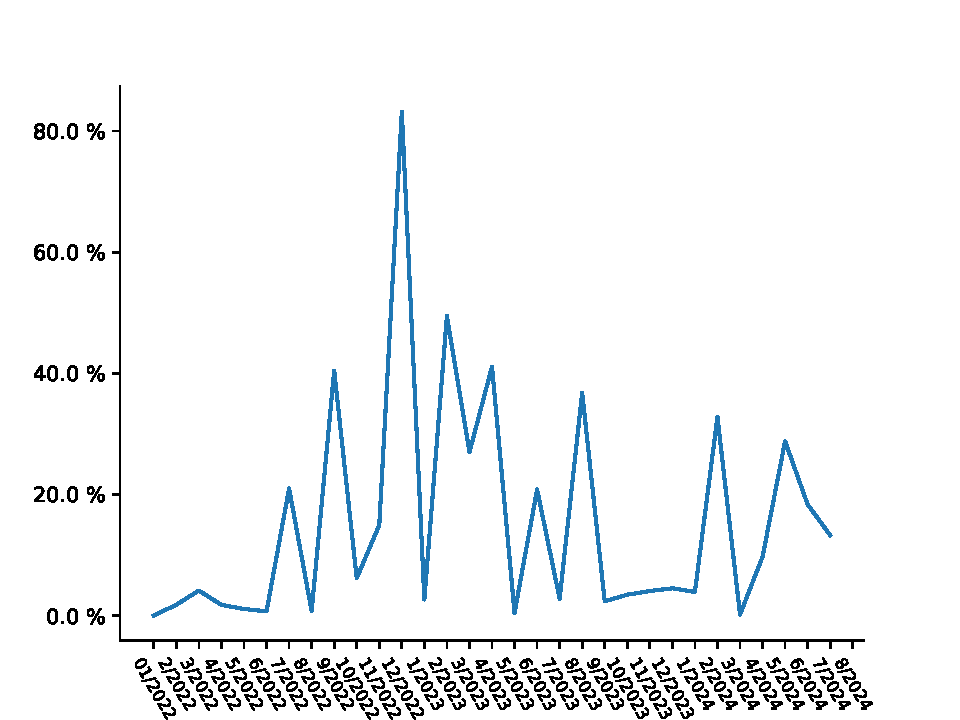
\includegraphics[width=\linewidth]{./chapters/4-results/packet-loss/img/NL.pdf}
		\caption{Netherlands}
	\end{subfigure}
	\begin{subfigure}[t]{0.47\linewidth}
		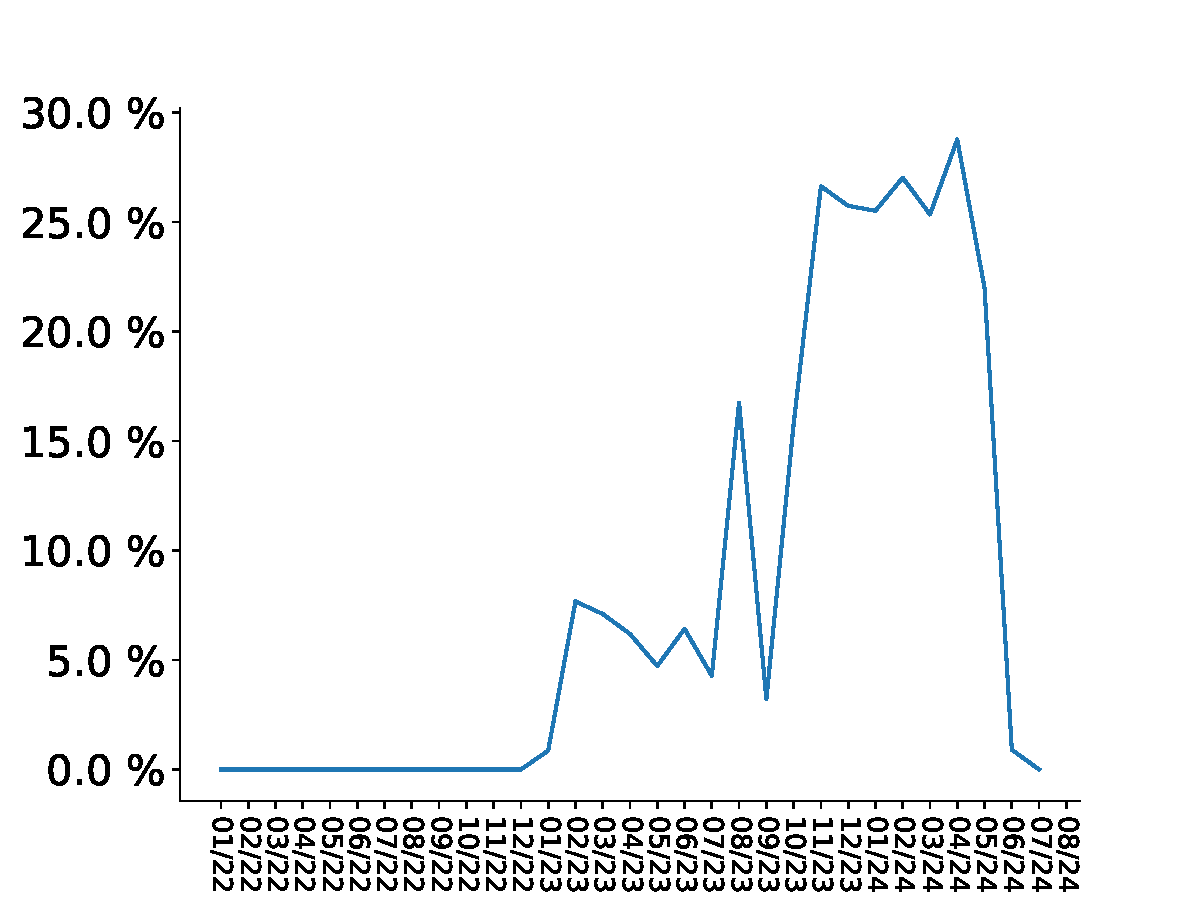
\includegraphics[width=\linewidth]{./chapters/4-results/packet-loss/img/PH.pdf}
		\caption{Philippines}
	\end{subfigure}
	\begin{subfigure}[t]{0.47\linewidth}
		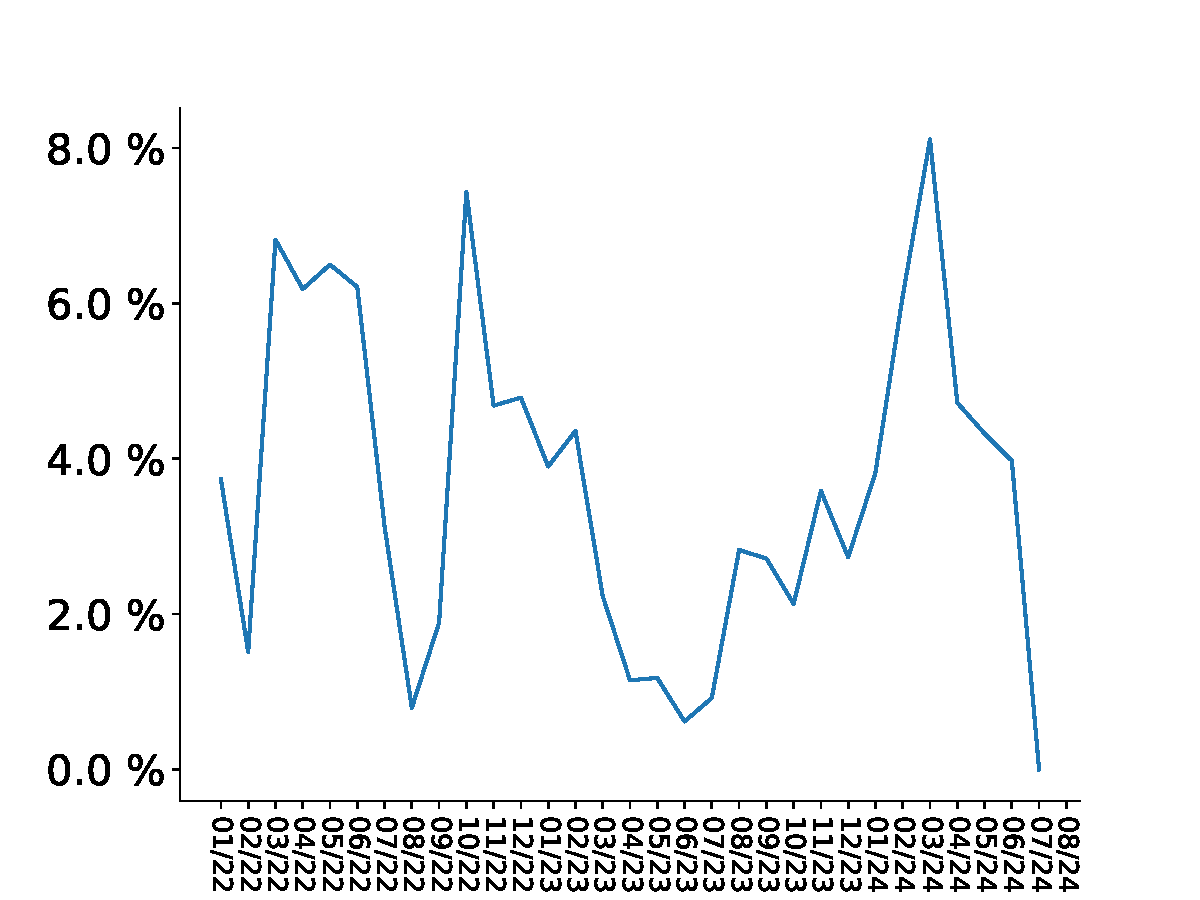
\includegraphics[width=\linewidth]{./chapters/4-results/packet-loss/img/US.pdf}
		\caption{USA}
	\end{subfigure}
	\caption{Packet Loss Ratios in Percent in individual Month from January
		2022 to June 2024}
	\label{fig:packet-loss-fine-grained}
\end{figure}

One can see that Germany experienced high volumes of packet loss in 2022
reaching as high as 40~\% packet loss in June 2022. This was followed by a
period of little packet loss ratios in 2023. Likely, papers taking measurements
at this time will report Germany to have very little packet loss. In 2024, the
trend is going back towards higher packet losses.

The Netherlands show fluctuating pattern that even reaches values of 80~\%
packet loss in December~2022. However, little conclusions can be made except
for the assumption that the connection is highly instable.

The Philippines only hold data since 2023. Therefore, we cannot make
conclusions about the packet loss in the Philippines in 2022. In 2023 however,
the packet loss was around five to eight percent, until in August 2023, the
packet loss rose to more than fifteen percent. In 2024, the packet loss even
rose above twenty-five percent. June 2024 saw a sudden reduction in packet
loss. However, there is to little time series data to determine whether this is
an outlier.

The USA shows a similar pattern to Germany. In 2022, the packet loss was
relatively high, followed by a reducion in 2023, followed by an increase in
2024. However, there are two key differences when comparing Germany and the
USA: (1) the USA experiences lower percentages in packet loss and (2) a
reduction of packet loss is suggested starting in April 2024, which does not
happen for Germany.

\begin{takeaway}{Packet Loss in Starlink}
	The packet loss of Starlink connections is for most countries in the
	range of 1~--~4 \%. However, there are major differences and regional
	proximity does not seem to play a role. Additionally, 2023 has
	experienced better packet loss results compared to 2022 and 2024. This
	is a key difference to the latency analysis, where 2023 has experienced
	the worst results. It seems that Starlink can only op optimize for
	either packet loss and latency. It is in question, whether both values
	correlate.
\end{takeaway}


\section{Latency Development on Individual Days} \label{sec:latency-individual-days}

We used the data to look at the latency development over a single data for individual days.
For that we used the built-in ping measurements taken in RIPE Atlas probes\footnote{Ping measurements are not representative for absolute numbers \cite{DBLP:conf/imc/PelsserCVB13}, but show a pattern.}.


\subsection{Latencies on Different Weekdays}
\label{sec:latency-weekdays}

It is in question whether TLS handshake latencies vary at different days of the
week. For example, the latency might be different comparing Mondays and
Sundays. To analyze that, we looked at RIPE~Atlas data and Cloudflare~Radar
data.

\subsubsection*{RIPE Atlas}

Using the RIPE Atlas data, we compare different weekdays over the time range of
2022 -- 2024. We were not able to find differences in individual weekdays.
Figure~\ref{fig:latencies-per-weekday} illustrates the latencies that occur in
each weekday as measured by the built-in TLS measurements.

\begin{figure}
	\centering
	\begin{subfigure}[b]{0.32\linewidth}
		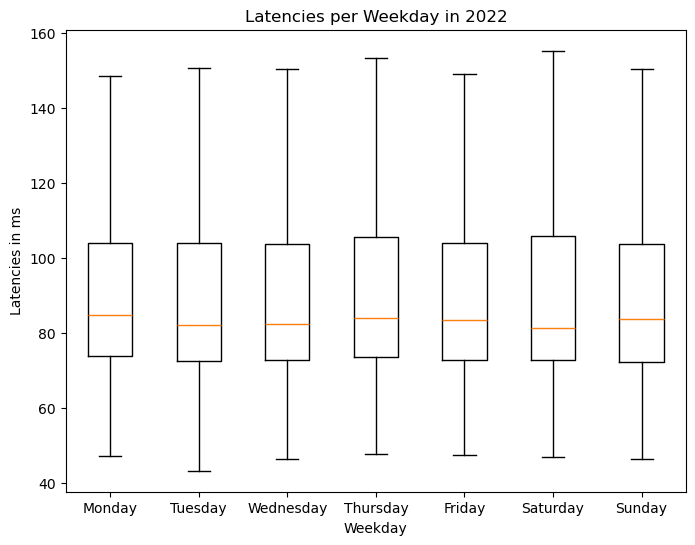
\includegraphics[width=\linewidth]{chapters/4-results/latency/img/latency_2022_weekdays.png}
	\end{subfigure}
	\begin{subfigure}[b]{0.32\linewidth}
		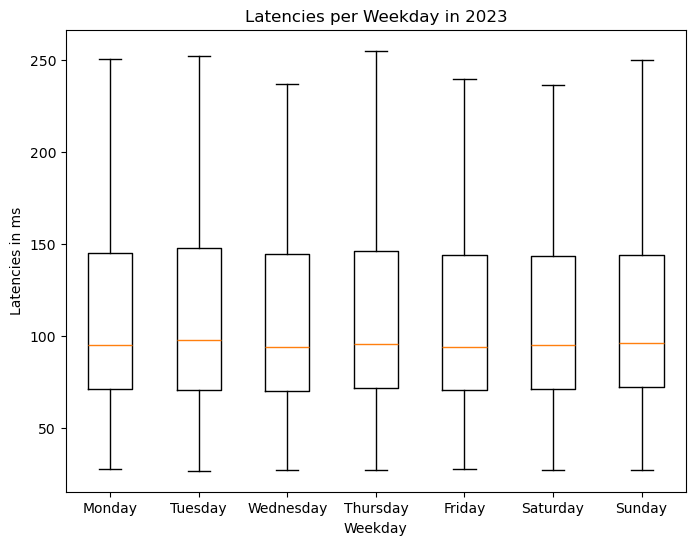
\includegraphics[width=\linewidth]{chapters/4-results/latency/img/latency_2023_weekdays.png}
	\end{subfigure}
	\begin{subfigure}[b]{0.32\linewidth}
		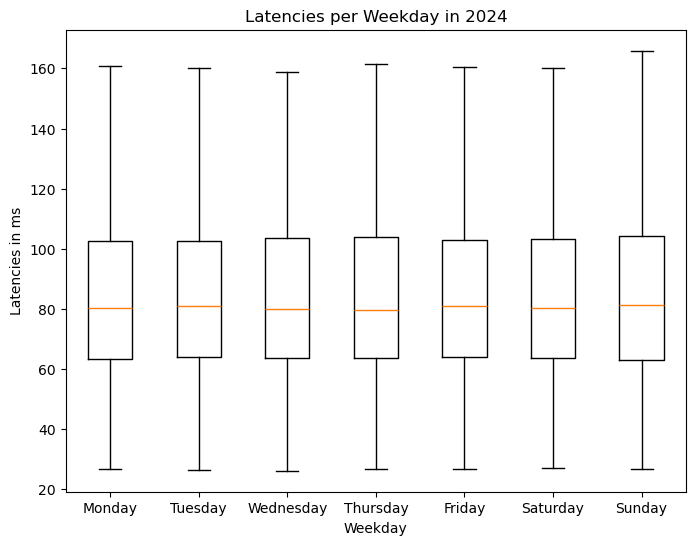
\includegraphics[width=\linewidth]{chapters/4-results/latency/img/latency_2024_weekdays.png}
	\end{subfigure}
	\caption{Latencies from 2022 to 2024 per Weekday.}
	\label{fig:latencies-per-weekday}
\end{figure}

One can see that there is no clear pattern that differentiates the individual
weekdays from the others. This does not change over the course of the years.

To look in more detail on the data, we looked at the data in specific
statistical aggregates (number of measurements, median, average, maximum, and
minimum latency). The results are shown in Table~\ref{fig:weekday-statistics}.

\begin{table}
	\begin{tabular}{llllllll}
		\toprule
		               & Mon. & Tue. & Wed. & Thu. & Fri. & Sat. & Sun. \\
		\midrule
		\textbf{2022}  &      &      &      &      &      &      &      \\
		\#Measurements & 899  & 895  & 904  & 903  & 906  & 918  & 893  \\
		Median         & 84   & 82   & 82   & 84   & 83   & 81   & 83   \\
		Average        & 100  & 100  & 106  & 97   & 99   & 99   & 93   \\
		Maximum        & 1211 & 3090 & 3056 & 703  & 1229 & 1106 & 672  \\
		Minimum        & 47   & 43   & 46   & 47   & 47   & 47   & 46   \\
		\midrule
		\textbf{2023}  &      &      &      &      &      &      &      \\
		\#Measurements & 1448 & 1447 & 1443 & 1429 & 1430 & 1436 & 1462 \\
		Median         & 95   & 98   & 94   & 95   & 94   & 95   & 96   \\
		Average        & 111  & 111  & 108  & 109  & 107  & 108  & 108  \\
		Maximum        & 1245 & 1227 & 1233 & 707  & 1088 & 1220 & 1052 \\
		Minimum        & 28   & 26   & 27   & 27   & 27   & 27   & 27   \\
		\midrule
		\textbf{2024}  &      &      &      &      &      &      &      \\
		\#Measurements & 914  & 930  & 904  & 913  & 914  & 912  & 918  \\
		Median         & 80   & 81   & 80   & 79   & 81   & 80   & 81   \\
		Average        & 97   & 93   & 104  & 105  & 95   & 95   & 95   \\
		Maximum        & 3147 & 1592 & 4374 & 3624 & 4368 & 1230 & 1320 \\
		Minimum        & 26   & 26   & 26   & 26   & 26   & 27   & 26   \\
		\bottomrule
	\end{tabular}
	\caption{Weekday Statistics in Germany}
	\label{fig:weekday-statistics}
\end{table}

They show that the latency does not vary on the individual days. Therefore, you
will not have a worse latency on working days (Monday -- Friday) compared to
the weekend (Saturday and Sunday).

However, the table also allows for an interesting comparison between the years
2022, 2023, and 2024. In 2022, the median TLS handshake latency was between 81
and 84 ms. The average latency was about 20 ms higher. Peak latencies achieved
up to 43 ms. In 2023, the median latencies were significantly higher at 94 to
98 ms. The average latency was in the worst case 14 ms higher, which indicates
a more stable connection, even if the performance was worse compared to 2022.
However, 2023 achieved much better peak performance at 26 ms. In 2024, Starlink
achieved similar median and average latencies compared to 2022, but also
achieving the peak performances from 2023.

\begin{takeaway}{Peak and Average Latency since 2022.}
	Starlink has managed to improve their peak latency by nearly 20 ms
	compared to 2022 while maintaining their median and average latencies.
\end{takeaway}

\subsubsection*{Cloudflare Radar}

Cloudflare offers a different perspective on the data as the data is acquired
differently. We use the Cloudflare Radar data to analyze how Starlink
performance changes over the course of a day. We do that with Cloudflare Radar
data as it offers aggregated data. Similar results are expected for RIPE~Atlas
measurements.





\section{Resilience of Networked Satellite Systems}

%
%	Resilience
%

% Disconnect Events
\subsection{Disconnect Events of RIPE Atlas Probes} \label{sec:disconnect-events}

Probes in RIPE Atlas automatically monitor the events when they are
disconnected from RIPE Atlas and when they re-connect again. Those disconnect
events give evidence about the state of a network. Frequently occurring
disconnect events might indicate an unhealthy network connection.

We analyzed the number of disconnect events for the Starlink probes in RIPE
Atlas. Figure~\ref{fig:disconnect-events-absolute} shows the number of
disconnect events per month in the time from January 2022 to July 2024.

\begin{figure}
	\centering
	\begin{subfigure}[b]{0.48\linewidth}
		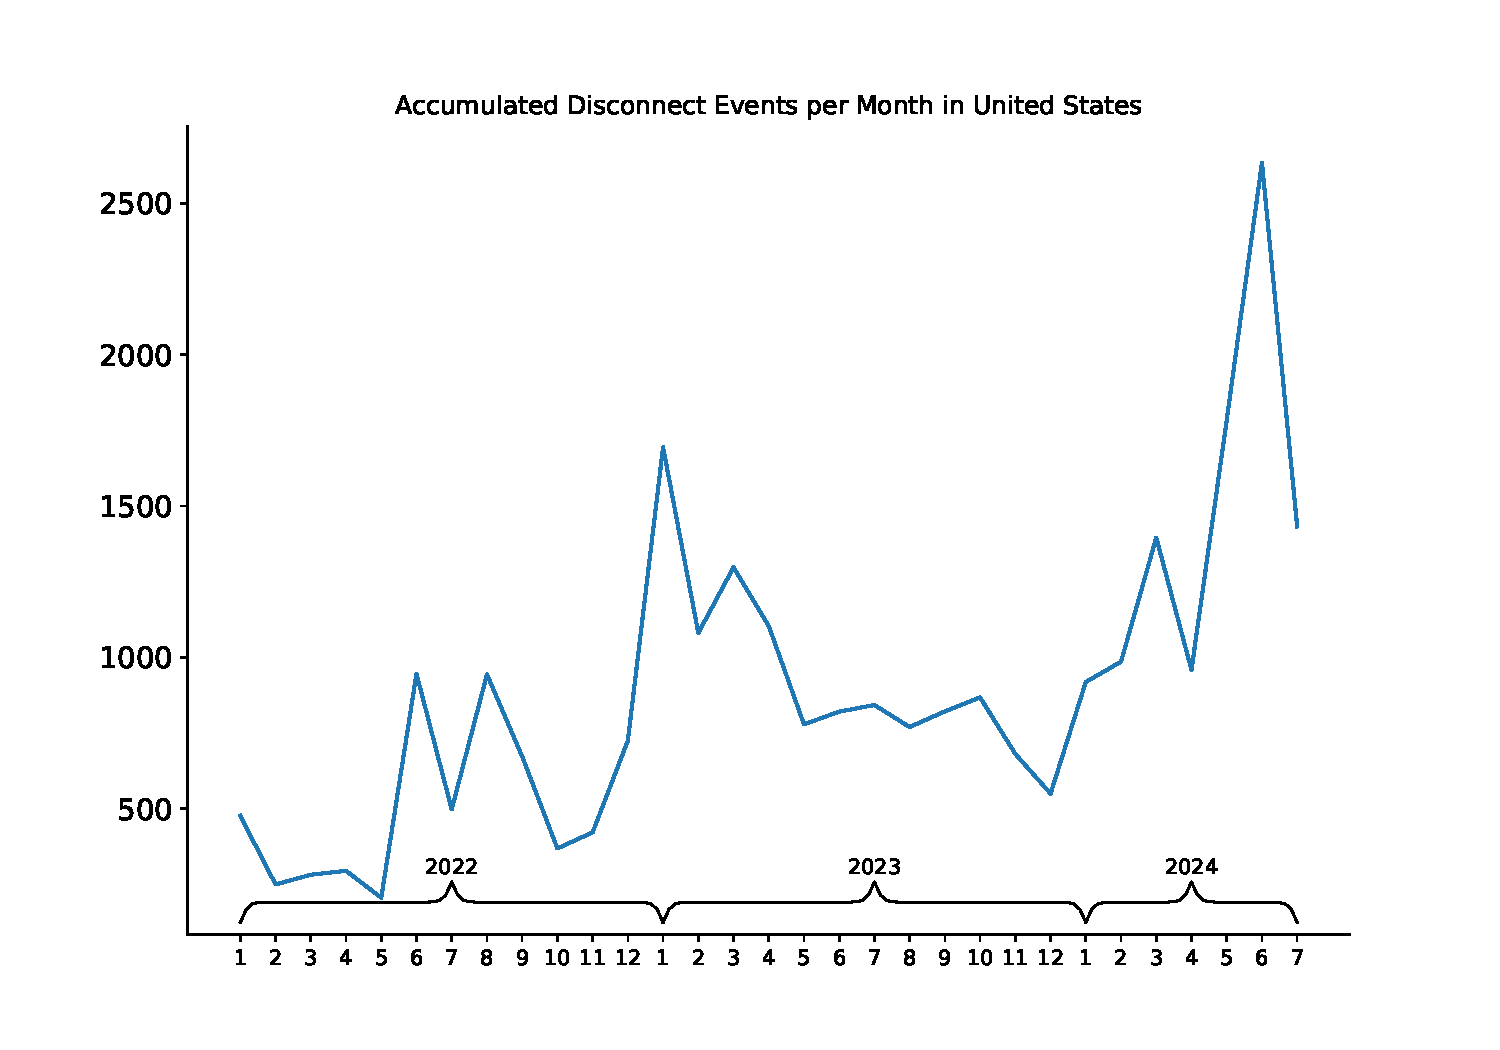
\includegraphics[width=\linewidth]{./chapters/4-results/disconnect_events/US.pdf}
		\caption{USA}
	\end{subfigure}
	\begin{subfigure}[b]{0.48\linewidth}
		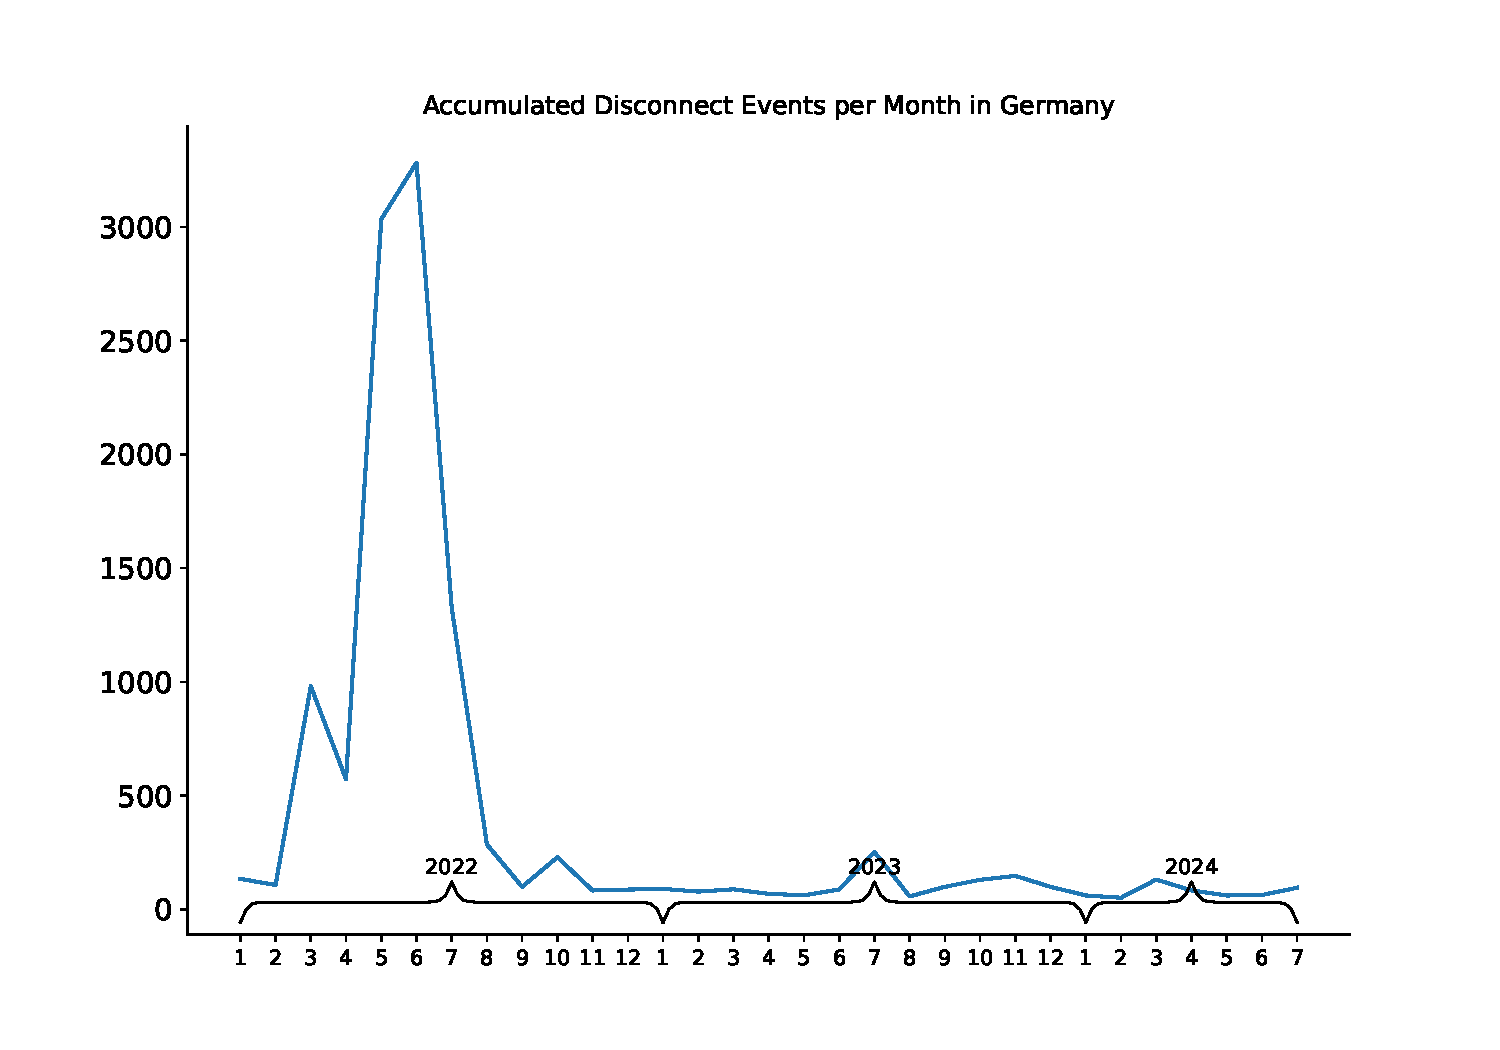
\includegraphics[width=\linewidth]{./chapters/4-results/disconnect_events/DE.pdf}
		\caption{Germany}
	\end{subfigure}
	\begin{subfigure}[b]{0.48\linewidth}
		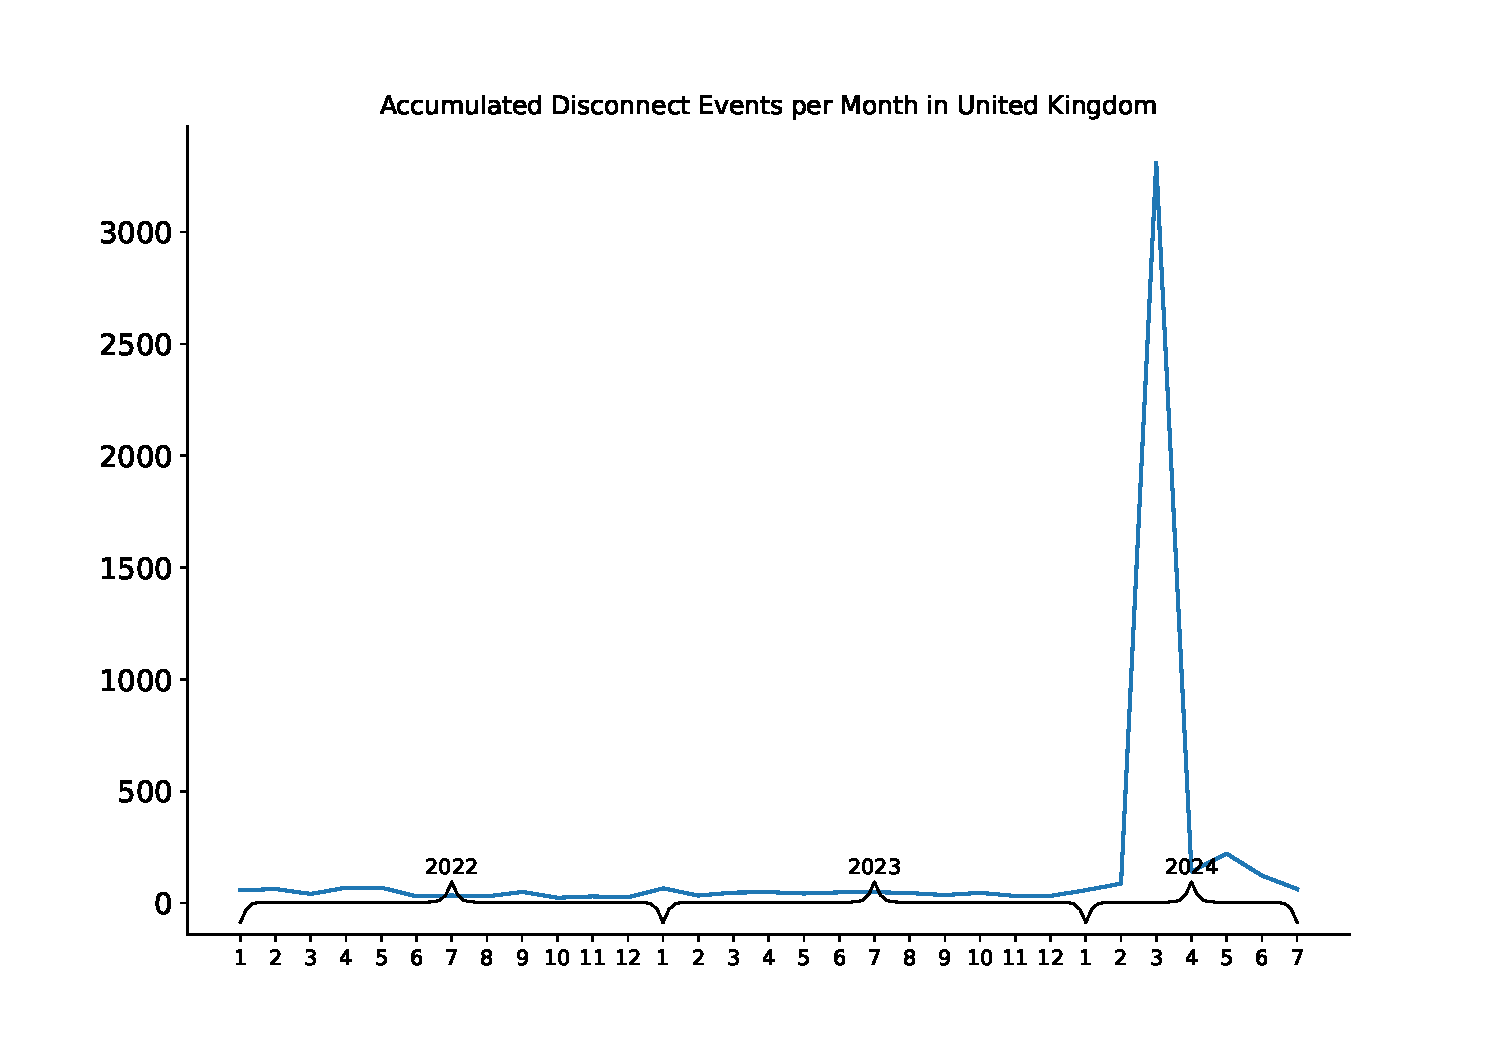
\includegraphics[width=\linewidth]{./chapters/4-results/disconnect_events/GB.pdf}
		\caption{United Kingdom}
	\end{subfigure}
	\caption{Number of Disconnect Events in the USA, Germany, and the
		United Kingdom from January 2022 to July 2024.}
	\label{fig:disconnect-events-absolute}
\end{figure}

One sees variously different patterns. While in Germany and the United Kingdom
very little disconnect events appear for the most time, the United States show
a relatively high number of disconnect events, increasing over time. The USA
experiences higher levels of disconnect events in June 2024, January 2023, and
May to August 2022. A clear pattern is not visible here. On the other side,
Germany experiences a high number of disconnect events in May to August 2022
(which also happens in the USA), while the United Kingdom does not show such a
behavior. The UK experiences a higher number of disconnect events in March
2024, but never before that. There is no clear pattern observable, when
comparing those three countries. A similar behavior was observed for other
countries.

Still, accumulating the number of disconnect events over all countries show
significant spikes. Figure~\ref{fig:disconnect-events-absolute-all-countries}
illustrates the pattern. Especially September and October 2023, the beginning
of 2024 and June 2024 show a much higher frequency. May and June 2022 have a
significant spike.

\begin{figure}
	\centering
	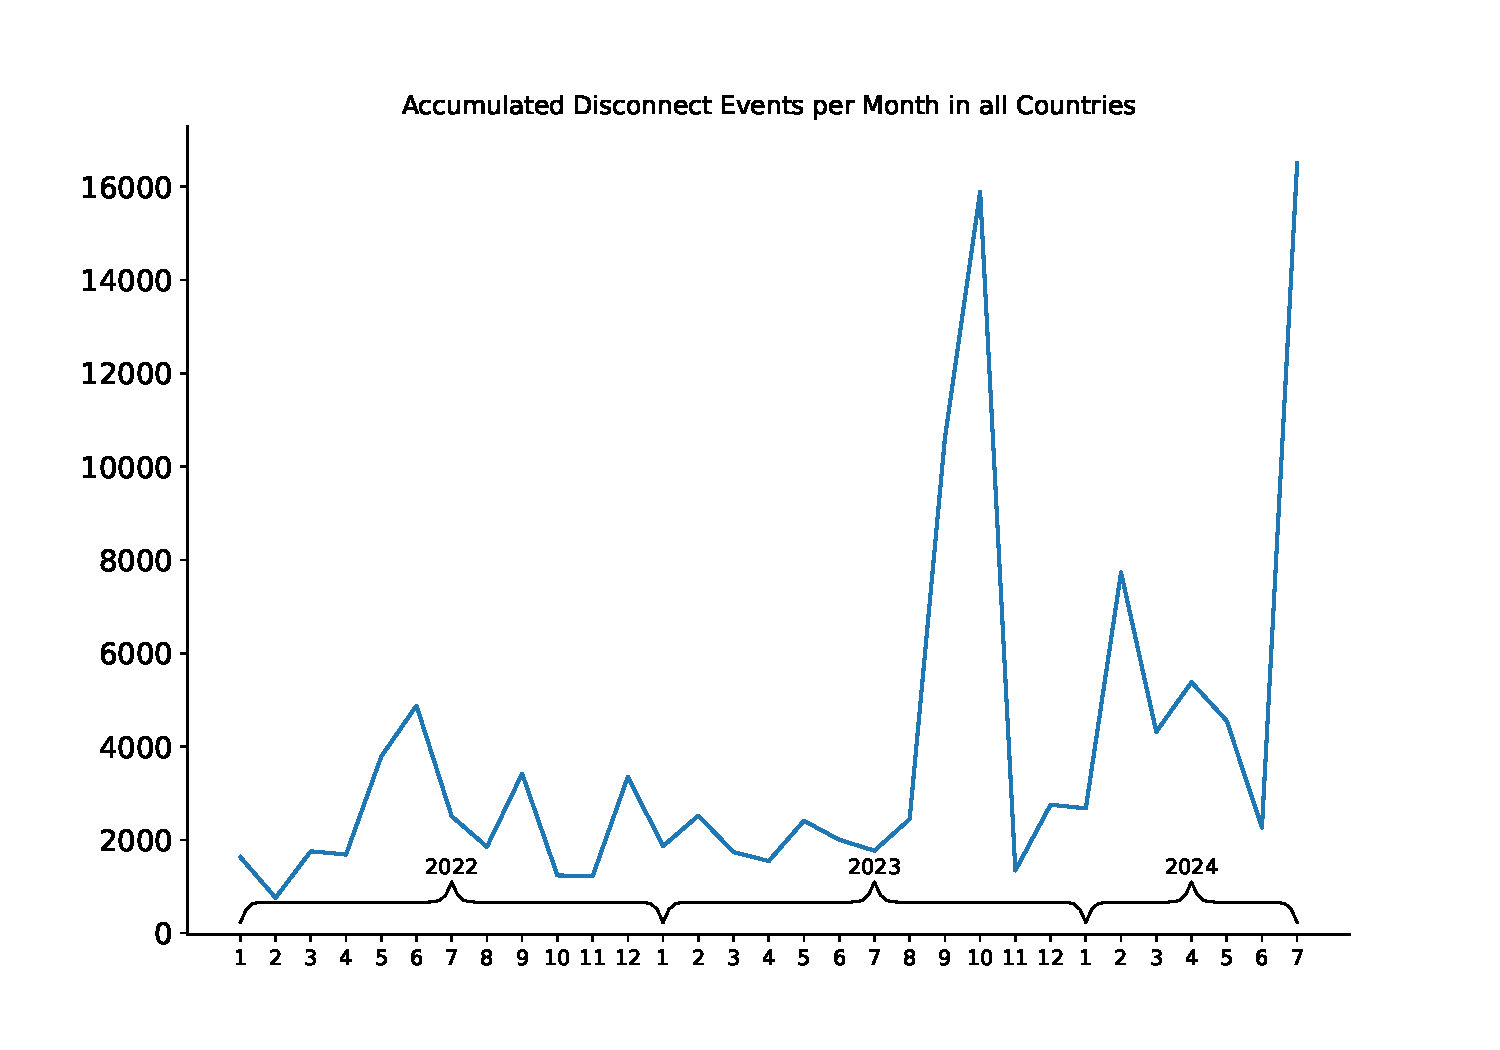
\includegraphics[width=.7\linewidth]{./chapters/4-results/disconnect_events/accumulated_disconnect_events_per_month_in_all_countries.pdf}
	\caption{Accumulated Number of Disconnect Events per Month in all
		Countries}
	\label{fig:disconnect-events-absolute-all-countries}
\end{figure}

We have to note that the data shown in
Figure~\ref{fig:disconnect-events-absolute-all-countries} does not allow making
conclusions. It holds different numbers of probes over time, so an increase in
disconnect events is expected. To draw conclusions for Starlink behavior, the
data needs to be normalized. Chapter~\ref{sec:correlation-disconnect-events}
explains this problem in more detail.

Also, the spikes in disconnection events may have been because of RIPE Atlas
system problems, which occur from time to time and cause many probes to
arbitrarily disconnect.

\begin{takeaway}{Usage of Disconnect Events}
	Accumulating Disconnect Events of Starlink probes seem to show a
	behavior that causes time intervals with higher occurrences. However,
	normalization is required to verify the observation. Normalization
	would be possible by using the active number of probes per time
	interval, but this was not done as it is not an easy task.
\end{takeaway}

\subsection*{Correlation of Disconnect Events with other Metrics}
\label{sec:correlation-disconnect-events}

One could correlate the occurrences of disconnect events with other metrics
(e.g., latencies and packet loss). Usually, this is done by comparing two
metrics with each other, where each metric is normalized. By normalizing, two
values of the same metric are comparable. In the case of disconnect events, the
number of disconnect events per time interval grows with the number of probes
connected. Therefore, the number of occurrences would be normalized by number
of probes connected.

However, the number of probes connected within a time interval is hard to find.
Some probes might be connected for a longer time than others dominating the
occurrences of disconnect events. Others might be connected for a very short
interval with many disconnects. Both scenarios compromise the normalization of
the disconnect event occurrences, leading to not meaningful results. It might
be well-possible to find a normalization method for disconnect events, but we
did not invest in this direction.

Therefore, we did not proceed further in correlating disconnect events with
other metrics.


% Correlation of Packet Loss and Latency
\section{Latency and Packet Loss Correlation} \label{sec:latency-packetloss-correlation}

Latency and packet loss are closely bonded. An increase of packet loss might
yield an increase in latency and vice-versa. For the data presented in the
previous chapter, we looked at the interval from January 2022 to June 2024. For
each month, we used the overall packet loss and the median latency. We used a
Pearson, Kendall, and Spearman correlation to determine possible correlations
between latency and packet loss. The results are shown in
Table~\ref{fig:packetloss-latency-correlation}.

\begin{table}[ht]
	\footnotesize
	\caption{Packet Loss and Latency Correlation}
	\label{fig:packetloss-latency-correlation}
	\begin{tabular}{lrrr}
		\toprule
		Country                     & Pearson     & Kendall     & Spearman    \\
		January 2022 - June 2024    & Correlation & Correlation & Correlation \\
		\midrule
		Falkland Islands (Malvinas) & 0.447641    & 0.595238    & 0.624282    \\
		Réunion                     & 0.636822    & 0.716314    & 0.847658    \\
		Kiribati                    & 0.819596    & 0.794851    & 0.801966    \\
		Canada                      & -0.090981   & 0.218391    & 0.280534    \\
		Poland                      & 0.093155    & -0.025287   & -0.073637   \\
		Haiti                       & 0.383601    & 0.670768    & 0.844964    \\
		Spain                       & -0.323940   & -0.163650   & -0.179434   \\
		Czechia                     & 0.700248    & 0.730392    & 0.806351    \\
		United States               & -0.556997   & -0.425287   & -0.610234   \\
		France                      & 0.893576    & 0.664368    & 0.840267    \\
		Italy                       & -0.073752   & 0.181609    & 0.293882    \\
		United Kingdom              & -0.238013   & -0.227586   & -0.279644   \\
		Honduras                    & 0.415387    & 0.410256    & 0.575585    \\
		Australia                   & -0.025590   & 0.013841    & 0.035834    \\
		Netherlands                 & 0.190923    & 0.055364    & 0.111952    \\
		Greece                      & 0.249727    & 0.496864    & 0.668590    \\
		Sweden                      & 0.678500    & 0.726984    & 0.896199    \\
		Austria                     & 0.054429    & 0.039080    & 0.073192    \\
		Belgium                     & -0.082786   & -0.029885   & -0.031368   \\
		Philippines                 & 0.254523    & 0.460118    & 0.676049    \\
		Virgin Islands, U.S.        & 0.712898    & 0.706384    & 0.878571    \\
		Germany                     & -0.787348   & -0.549425   & -0.753059   \\
		\bottomrule
	\end{tabular}
\end{table}

In a correlation, a value close to 1 or -1 shows a strong correlation. Values
close to 0 do not appear to be correlated. In the results, some countries show
a correlation, e.g., France or Czechia. Other countries, e.g., Canada or
Australia do not show correlating values. As the number of countries with a
stronger and those with a weaker correlation is equally distributed, we cannot
conclude a correlation between latency and packet loss in Starlink networks.

\subsection{Correlation in Single Years}

Analyzing single years give a better understanding of the development of
correlation in the year 2022, 2023, and 2024 (until June). The
Tables~\ref{fig:packetloss-latency-correlation-2022},
\ref{fig:packetloss-latency-correlation-2023}, and
\ref{fig:packetloss-latency-correlation-2024} show the individual correlation
values for the year. There are only countries displayed, where a correlation
value could be calculated.

\begin{table}
	\footnotesize
	\caption{Packet Loss and Latency Correlation in 2022}
	\label{fig:packetloss-latency-correlation-2022}
	\begin{tabular}{lrrr}
		\toprule
		Country        & Pearson     & Kendall     & Spearman    \\
		2022           & Correlation & Correlation & Correlation \\
		\midrule
		Canada         & 0.478988    & 0.272727    & 0.307692    \\
		Poland         & 0.601734    & 0.303030    & 0.342657    \\
		Spain          & -0.286931   & -0.053571   & -0.037594   \\
		United States  & -0.241717   & -0.212121   & -0.363636   \\
		France         & 0.177126    & -0.060606   & -0.083916   \\
		Italy          & 0.646487    & 0.484848    & 0.587413    \\
		United Kingdom & 0.514397    & 0.363636    & 0.496503    \\
		Honduras       & 0.208592    & -0.333333   & -0.426573   \\
		Australia      & 0.870466    & 0.325669    & 0.450715    \\
		Netherlands    & 0.159295    & -0.106873   & -0.164624   \\
		Greece         & 0.811845    & 0.836660    & 0.853766    \\
		Austria        & 0.013609    & -0.060606   & -0.146853   \\
		Belgium        & -0.283806   & -0.242424   & -0.272727   \\
		Germany        & -0.663075   & -0.303030   & -0.517483   \\
		\bottomrule
	\end{tabular}
\end{table}

\begin{table}
	\footnotesize
	\caption{Packet Loss and Latency Correlation in 2023}
	\label{fig:packetloss-latency-correlation-2023}
	\begin{tabular}{lrrr}
		\toprule
		Country                     & Pearson     & Kendall     & Spearman    \\
		2023                        & Correlation & Correlation & Correlation \\
		\midrule
		Falkland Islands (Malvinas) & 0.364389    & 0.466667    & 0.518072    \\
		Réunion                     & 0.587427    & 0.467801    & 0.592125    \\
		Canada                      & 0.370590    & 0.363636    & 0.608392    \\
		Poland                      & -0.261476   & -0.090909   & -0.216783   \\
		Haiti                       & 0.757392    & 0.390673    & 0.529108    \\
		Spain                       & -0.413832   & -0.160714   & -0.218045   \\
		Czechia                     & 0.415844    & 0.383333    & 0.458333    \\
		United States               & -0.302660   & -0.242424   & -0.251748   \\
		France                      & 0.779247    & 0.666667    & 0.818182    \\
		Italy                       & -0.568765   & -0.272727   & -0.412587   \\
		United Kingdom              & -0.812772   & -0.606061   & -0.748252   \\
		Honduras                    & 0.343476    & 0.516667    & 0.617754    \\
		Australia                   & -0.578546   & -0.121212   & -0.258741   \\
		Netherlands                 & 0.212359    & 0.181818    & 0.314685    \\
		Greece                      & -0.268072   & 0.212121    & 0.195804    \\
		Sweden                      & 0.515385    & 0.533333    & 0.717391    \\
		Austria                     & -0.294406   & -0.121212   & -0.125874   \\
		Belgium                     & 0.441123    & 0.454545    & 0.573427    \\
		Philippines                 & -0.196523   & -0.030303   & -0.034965   \\
		Virgin Islands, U.S.        & 0.553108    & 0.578196    & 0.783080    \\
		Germany                     & -0.620018   & -0.424242   & -0.622378   \\
		\bottomrule
	\end{tabular}
\end{table}

\begin{table}
	\footnotesize
	\caption{Packet Loss and Latency Correlation in 2024}
	\label{fig:packetloss-latency-correlation-2024}
	\begin{tabular}{lrrr}
		\toprule
		Country              & Pearson     & Kendall     & Spearman    \\
		2024                 & Correlation & Correlation & Correlation \\
		\midrule
		Réunion              & 0.301680    & -0.066667   & -0.085714   \\
		Kiribati             & 0.744916    & 0.673575    & 0.718421    \\
		Canada               & -0.003851   & -0.600000   & -0.771429   \\
		Poland               & 0.239930    & 0.333333    & 0.371429    \\
		Haiti                & 0.376160    & 0.200000    & 0.257143    \\
		Spain                & -0.044513   & -0.333333   & -0.142857   \\
		United States        & -0.529555   & -0.600000   & -0.771429   \\
		France               & 0.418669    & 0.200000    & 0.257143    \\
		Italy                & -0.600898   & -0.866667   & -0.942857   \\
		United Kingdom       & 0.243811    & 0.333333    & 0.428571    \\
		Honduras             & 0.431954    & 0.333333    & 0.542857    \\
		Australia            & -0.155578   & -0.066667   & -0.085714   \\
		Netherlands          & 0.433624    & 0.466667    & 0.542857    \\
		Greece               & -0.813812   & -0.466667   & -0.600000   \\
		Sweden               & 0.280194    & 0.066667    & 0.085714    \\
		Austria              & 0.915449    & 0.466667    & 0.600000    \\
		Belgium              & 0.428515    & 0.333333    & 0.371429    \\
		Philippines          & -0.920833   & -0.466667   & -0.428571   \\
		Virgin Islands, U.S. & -0.450938   & -0.333333   & -0.428571   \\
		Germany              & -0.603772   & -0.333333   & -0.485714   \\
		\bottomrule
	\end{tabular}
\end{table}

In 2022, there was little correlation at all. Likely, other factors like
satellite infrastructure or presence of \ac{PoP} might have been more
contributing to performance issues. 2023 showed a stronger correlation compared
to 2022. We assume that this is due to a more stable network. The interaction
between packet loss and latency might have become more significant. In 2024,
the correlation decreased once again slightly. This behavior is similar to the
one observed for the latencies in recent months. A possible explanation for
that is a growing user base of Starlink leading to a congestion of the system.
It has to be noted that the growth of number of satellites did not increase
from 2023 to 2024 as much as it did from 2022 to 2023, which might be a cause
of the issue.

\subsection{Correlation with the Number of Probes} \label{sec:number-of-probes-correlation}

It is possible that the data is insufficient resulting in a correlation between
latency and packet loss being invisible. A possibility is to look at the number
of probes being available for each country. Therefore, we took the data from
Table~\ref{fig:packetloss-latency-correlation} and correlated it with the
number of probes available for RIPE Atlas in each country. The resulting table
is shown in Figure~\ref{fig:packetloss-latency-number-probes-correlation}.

\begin{table}[ht]
	\footnotesize
	\caption{Packet Loss, Latency and Number of Probes Correlation}
	\label{fig:packetloss-latency-number-probes-correlation}
	\begin{tabular}{lrrrr}
		\toprule
		Country               & Pearson     & Kendall     & Spearman    & Number of \\
		Jan. 2022 - June 2024 & Correlation & Correlation & Correlation & Probes    \\
		\midrule
		Falkland Islands      & 0.447641    & 0.595238    & 0.624282    & 1         \\
		(Malvinas)                                                                  \\
		Réunion               & 0.636822    & 0.716314    & 0.847658    & 1         \\
		Kiribati              & 0.819596    & 0.794851    & 0.801966    & 2         \\
		Canada                & -0.090981   & 0.218391    & 0.280534    & 11        \\
		Poland                & 0.093155    & -0.025287   & -0.073637   & 1         \\
		Haiti                 & 0.383601    & 0.670768    & 0.844964    & 3         \\
		Spain                 & -0.323940   & -0.163650   & -0.179434   & 4         \\
		Czechia               & 0.700248    & 0.730392    & 0.806351    & 1         \\
		United States         & -0.556997   & -0.425287   & -0.610234   & 53        \\
		France                & 0.893576    & 0.664368    & 0.840267    & 18        \\
		Italy                 & -0.073752   & 0.181609    & 0.293882    & 4         \\
		United Kingdom        & -0.238013   & -0.227586   & -0.279644   & 11        \\
		Honduras              & 0.415387    & 0.410256    & 0.575585    & 1         \\
		Australia             & -0.025590   & 0.013841    & 0.035834    & 8         \\
		Netherlands           & 0.190923    & 0.055364    & 0.111952    & 2         \\
		Greece                & 0.249727    & 0.496864    & 0.668590    & 1         \\
		Sweden                & 0.678500    & 0.726984    & 0.896199    & 1         \\
		Austria               & 0.054429    & 0.039080    & 0.073192    & 4         \\
		Belgium               & -0.082786   & -0.029885   & -0.031368   & 2         \\
		Switzerland           & NaN         & NaN         & NaN         & 1         \\
		Philippines           & 0.254523    & 0.460118    & 0.676049    & 3         \\
		Benin                 & NaN         & NaN         & NaN         & 2         \\
		Virgin Islands, U.S.  & 0.712898    & 0.706384    & 0.878571    & 1         \\
		Germany               & -0.787348   & -0.549425   & -0.753059   & 10        \\
		\bottomrule
	\end{tabular}
\end{table}

We correlated the correlation values with the number of probes per country.
This resulted in the following correlation values:

\begin{itemize}
	\item Pearson Correlation: $\approx -0.44$
	\item Kendall Correlation: $\approx -0.44$
	\item Spearman Correlation: $\approx -0.53$
\end{itemize}

As the correlation does not reach values close to 0, 1, or -1, we cannot
conclude a correlation with the number of probes.

\begin{takeaway}{The correlation of latency and packet loss.}
	Starlink does not show a clear pattern that indicates a correlation
	between latency and packet loss. However, this is highly dependent on
	the country of origin.
\end{takeaway}


% Routing
% last-modified: 08.08.2024
% how-to-reproduce: /src/db-controller/notebooks/traceroute.ipynb

\section{Traceroute Analysis} \label{sec:traceroute-analysis}

Looking at traceroute results, we can make conclusions about the routing behavior of Starlink network devices. In the data we gathered more than forty million traceroute measurements. Those include primarily built-in measurements from RIPE Atlas probes to \textit{*.root-servers.net} for Starlink probes (\ac{ASN} 14593).

\subsection*{Routing Behavior}

\begin{figure}
	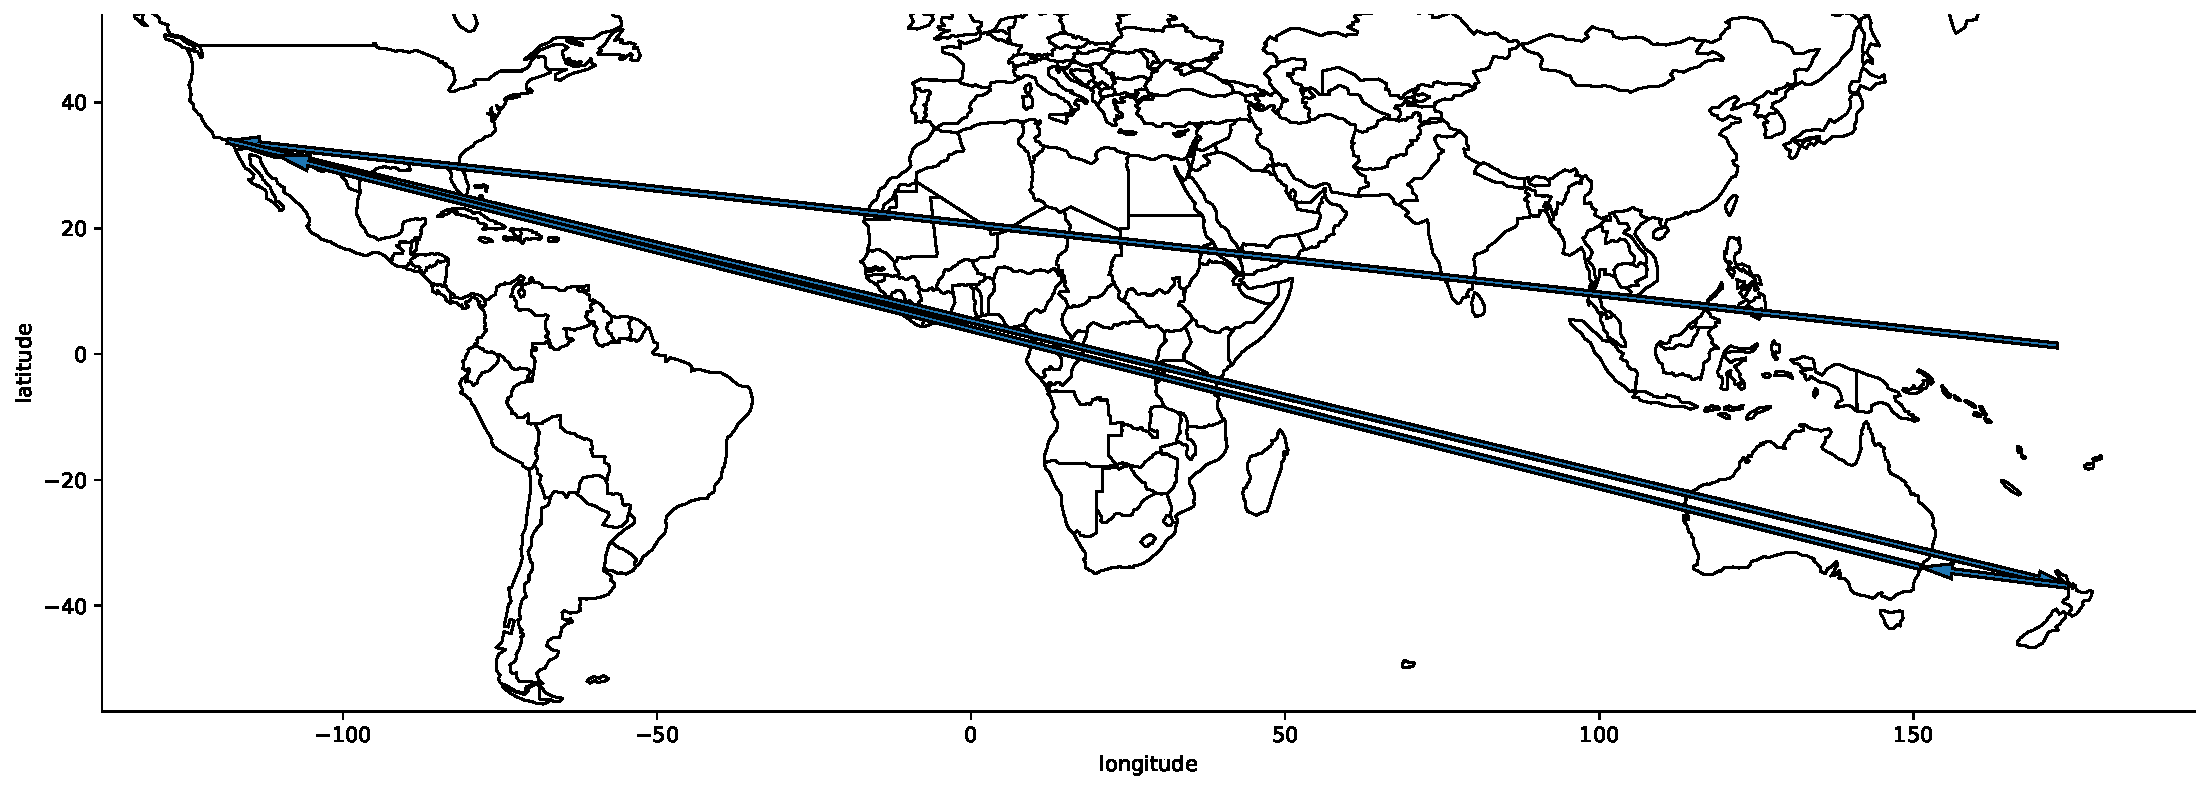
\includegraphics[width=\textwidth]{chapters/4-results/img/kiribati-example-traceroute.pdf}
	\caption{Visualization of a Traceroute from Kiribati}
	\label{fig:kiribati-example-traceroute}
\end{figure}

First, we found that the satellite hops are likely invisible to the traceroute. We conclude that as there are no hops visible above water, even for probes located in remote regions, e.g., Kiribati in the Pacific Ocean. In Figure~\ref{fig:kiribati-example-traceroute}, one can see a visualization of a traceroute result from Kiribati to \textit{f.root-servers.net}. One can see that the first visible hop is located in New~Zealand or an island to the north of New~Zealand. However, if satellites were visible, we'd be able to observe more satellites.

% TODO: Cite the statement that 4000km is too large for a single satellite. Everybody would ask here now: "But how much can they actually cover?"
Coming from the first insight, we can also conclude that \ac{ISLs} are enabled. If they were not, we would likely not be able to see a successful traceroute from Kiribati to a location. The next closest known \ac{PoP} is on Hawaii. However, the distance between both is 4000~km, which is more than a single satellite can cover. Aside from that, we do not observe the usage of the \ac{PoP} in Hawaii, but in more distant locations, which just strengthens the argument. Therefore, we conclude that \ac{ISLs} are enabled. This is special interest, as it was not clear in recent research \cite{Hauri2020}.

\subsection{Privacy Concerns in Traceroute Data}

One of the most important responsibilities of an \ac{ISP} is to ensure the privacy of its users. This also includes to route traffic only in trusted countries. In the case of Starlink, we were able to observe a different behavior. We looked at a slice of the built-in traceroute measurements from German Starlink probes and analyzed their most common targets. We filtered for anycasted servers (e.g., *.root-servers.net) and bogon IPs (i.e., IPs that cannot be associated with metadata).

% Input IP Hitlist
\begin{table}
	\caption{IP Hitlist for Built-In Traceroute Measurements}
	\label{fig:ip-hitlist-traceroute}
	\begin{tabular}{rllll}
		\toprule
		Hits  & City              & Country       & Organization & IP Address      \\
		\midrule
		10634 & Frankfurt am Main & Germany       & AS1299       & 62.115.37.20    \\
		8202  & Offenbach         & Germany       & Unknown      & 80.81.192.154   \\
		6207  & Amsterdam         & Netherlands   & Unknown      & 193.239.116.217 \\
		5582  & Frankfurt am Main & Germany       & AS2914       & 213.198.72.18   \\
		5257  & Frankfurt am Main & Germany       & AS3257       & 89.149.137.14   \\
		4932  & Chicago           & United States & AS14593      & 206.224.65.178  \\
		4916  & Chicago           & United States & AS14593      & 206.224.65.180  \\
		4850  & Chicago           & United States & AS14593      & 206.224.65.182  \\
		4755  & Chicago           & United States & AS14593      & 206.224.65.184  \\
		4358  & Miami             & United States & AS49791      & 81.31.213.126   \\
		4333  & Zürich            & Switzerland   & Unknown      & 185.1.147.30    \\
		4256  & Tokyo             & Japan         & Unknown      & 210.173.176.242 \\
		4179  & Chicago           & United States & AS14593      & 206.224.65.186  \\
		4035  & Chicago           & United States & AS14593      & 206.224.65.192  \\
		4014  & Frankfurt am Main & Germany       & AS6762       & 213.144.184.30  \\
		4010  & Chicago           & United States & AS14593      & 206.224.65.190  \\
		4005  & Chicago           & United States & AS14593      & 206.224.65.188  \\
		4002  & Frankfurt am Main & Germany       & AS1299       & 62.115.124.118  \\
		3990  & Singapore         & Singapore     & AS2497       & 202.232.1.69    \\
		3827  & Frankfurt am Main & Germany       & AS6939       & 72.52.92.70     \\
		\bottomrule
	\end{tabular}
\end{table}

In Table~\ref{fig:ip-hitlist-traceroute}, the top twenty most frequent hits of IP addresses are shown. The IP addresses are joined with data from IPInfo. As traffic goes from a German probe to an anycasted server, located in Germany, one would expect little traffic outside Germany, and none outside Europe. The top five IP addresses are located within or close to Germany, but the next five already involve traffic to the United~States. Here, we observe an unexpected behavior. Assuming that the data is not flawed, this is a clear violation of guiding privacy principles.



% Limitations and Future Work
%	- Limitation of Probe Availability (only selected ones on RIPE Atlas)
%	- Limitation of Service Availability (Starlink only)
%	- Limitation of IPInfo Database
%	- Limitation of Black-Box approach (no insight in Starlink intrinsics)

% Conclusion
\chapter{Conclusions \& Outlook}
\chapter{Conclusions \& Outlook} \label{sec:conclusion}

We have looked at the performance and resilience of the Starlink satellite
system. The main research questions are listed in
Chapter~\ref{sec:research-questions}.

To answer research question 1, we looked at the TLS handshake latency in each
years 2022~--~2024 and found that Starlink latency is at approximately 80~ms
median in 2024. However, it has to be noted that Starlink latency improved
since 2022 in average, median, and minimal latency (see
Table~\ref{fig:weekday-statistics}).

We observed a strange behavior in the latency that we call the
"two-bell-pattern." It is visible in Figure~\ref{fig:latency-histogram-1} and
\ref{fig:latency-histogram-2}. It describes the behavior of serving two ranges
of latencies especially well. First lower latencies ($\approx$~80~--100~ms) and
second higher latencies ($\approx$~150~--250~ms) with a major gap in between.
The cause of this pattern is unclear.

Additionally, we wanted to find out about diurnal variation. Looking at data
from April~2024, we found that there is no difference between the individual
week days (see Figure~\ref{fig:latencies-per-weekday}). However, there is a
strong variation between the hours of the day. For example, one can expect
lower latencies at night compared to during lunchtime.

We also looked at packet loss and noted a high variation by country. Countries
such as the Philippines have packet loss ratios of up to 18\%, while Czechia
and Chile achieve less than 0.25\%. On the other hand side, highly modernized
countries like Germany and the Netherlands experience high packet loss ratios
(see Table~\ref{fig:packetloss-total}). Overall, most countries have a packet
loss of 1 to 4\%.

We expected a correlation in packet loss and latency and therefore correlated
them. We split the values by year and by country.
Table~\ref{fig:packetloss-latency-correlation} shows the resulting correlation
values, where 0 indicates orthogonal random variables and 1 or -1 indicates a
strong correlation. Some countries hold values that allow to draw a conclusion,
but others do not. We assumed that the number of probes played a role, but were
able to eliminate it as a determinant of behavior (see
Table~\ref{fig:packetloss-latency-number-probes-correlation}). The correlation
might be related to currently unknown contributing factors that need to be
taken into consideration before drawing a conclusion. Therefore, we cannot make
a statement about the correlation of latency and packet loss. Research question
2 can consequently not be answered by our research.

To answer research question 3, we further looked at the routing of the Starlink
satellite system. First, we wanted to find out the number of hops a route
usually takes. We found that most routes take 10 to 14 hops (see
Figure~\ref{fig:hops-per-measument}). The histogram for the hops also shows the
mentioned "two-bell-pattern." Both observations might be related, which was not
further researched in this thesis.

We also observed the change in latency per hop (i.e., what the traceroute
measurement latency reports in each hop). We found that usually there is a
spike in latency in the second hop. Likely, the spike originates from routing
through the Starlink satellite constellation, which is not reflected in the
traceroute results (see Figures~\ref{fig:latency-change-per-hop-1} and
\ref{fig:latency-change-per-hop-2}). We also found consequent spikes in
latency. However, in mapping the hops to their predominant ASN, we found that
those spikes lay outside the Starlink domain. Starlink has an opportunity of
improving its performance at this point, but likely other entities are actually
responsible for the spike.

Finally, we looked at the influence of solar magnetic storms on the Starlink
latency and found that there is no correlation (i.e., both random
variables are orthogonal).

\section{Future Work}

During our work, we faced several limitations that required more effort. The
first limitation were the probes that we did not hold ourselves, but which
originate from RIPE~Atlas. This means unknown people in the world set them up
as they wished. This might have corrupted the data. Ideally, the probes are
operated by the researchers themselves, but doing this a costly and tedious
undertaking.

Further, some directions were left unexplored due to time constraints. The
two-bell-pattern is an interesting observation that needs confirmation and
explanation as it was not clear why it occurred. It should also be correlated
with the similar observation in number of hops.

A detailed look at how Starlink routes packets on its satellite constellation
and later in terrestrial internet is left out. It is clear that Starlink cannot
give away complete responsibility after a packet is handed to a different AS.
At the same time, a proper model for such a routing behavior is missing.
Certain parts, like the placing of ground stations, are known, but a complete
model was not yet found.

Mentioned in Chapter~\ref{sec:bent-pipes}, \ac{SNO}s largely rely on \ac{ISL}s.
Looking at the traceroute data, it is obvious that \ac{ISL}s are used for
supporting remote regions. In parallel, research discusses the impact of
\ac{ISL}s on the performance. Their impact and ideal usage are questions that
need to be addressed and are a matter of future research.



% Appendix
\chapter{Appendix}
\begin{figure}
	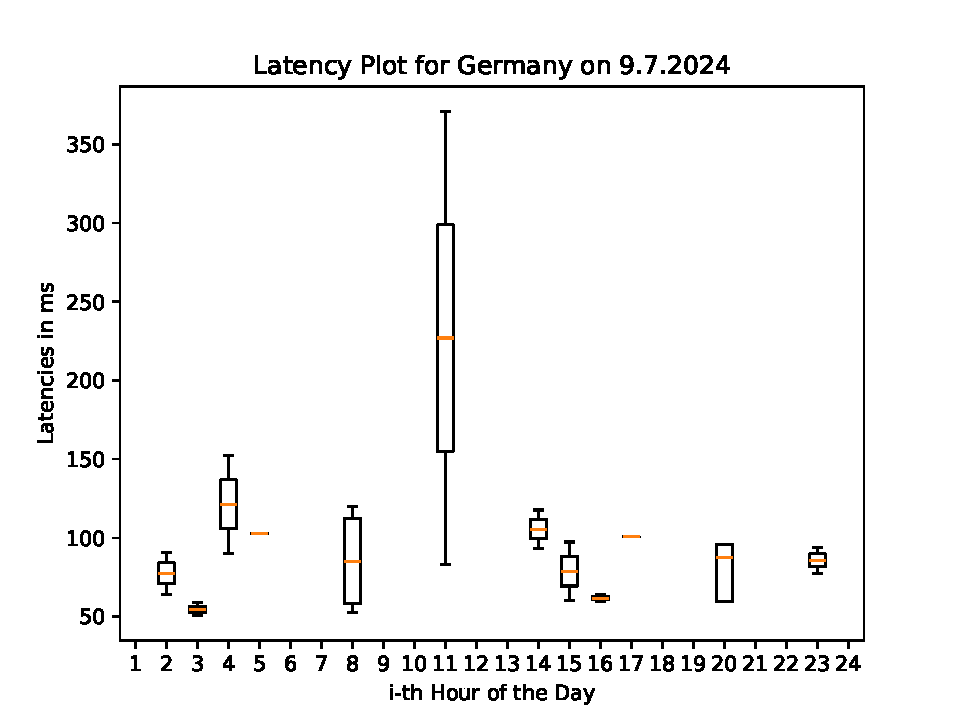
\includegraphics[width=\textwidth]{./chapters/appendix/img/latency_plot_for_germany_on_9.7.2024.pdf}
	\caption{Latency over the July 9, 2024 using TLS data.}
	\label{fig:tls-analysis-individual-day}
\end{figure}

\begin{figure}
	\centering
	\begin{subfigure}[b]{0.48\linewidth}
		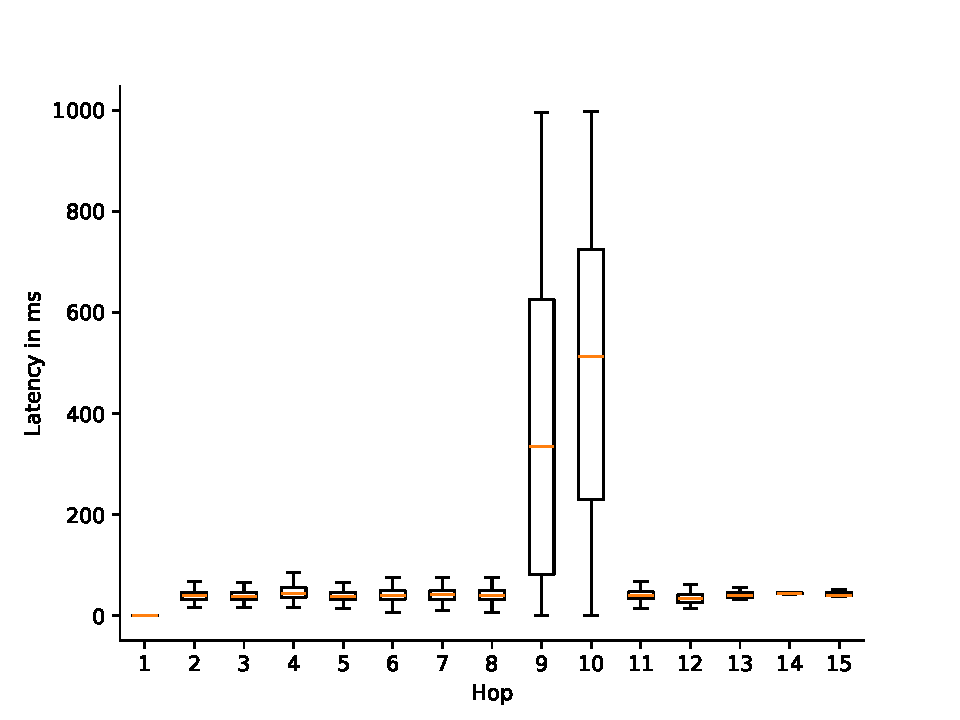
\includegraphics[width=\linewidth]{chapters/4-results/traceroute/img/latency-per-hop-PL.pdf}
		\caption{Poland}
	\end{subfigure}
	\begin{subfigure}[b]{0.48\linewidth}
		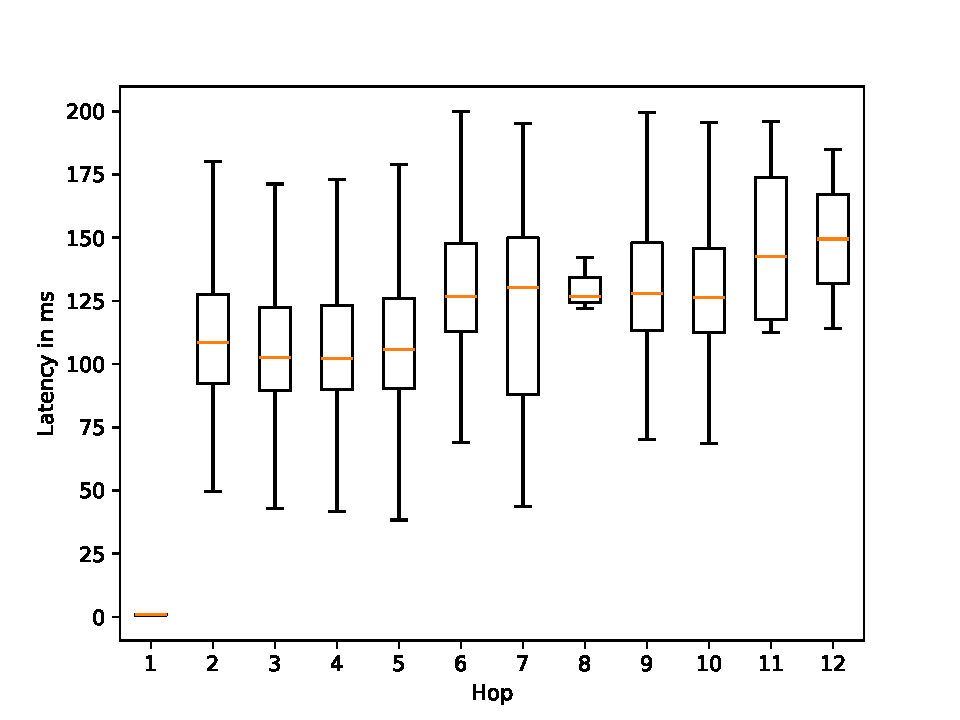
\includegraphics[width=\linewidth]{chapters/4-results/traceroute/img/latency-per-hop-KI.pdf}
		\caption{Kiribati}
	\end{subfigure}
	\begin{subfigure}[b]{0.48\linewidth}
		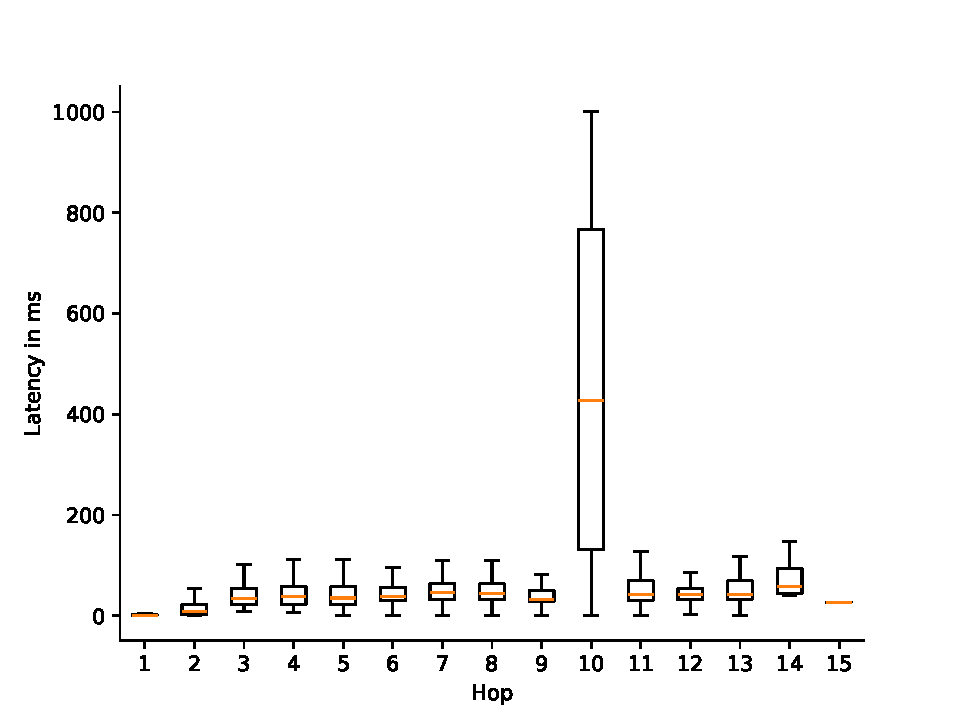
\includegraphics[width=\linewidth]{chapters/4-results/traceroute/img/latency-per-hop-IT.pdf}
		\caption{Italy}
	\end{subfigure}
	\begin{subfigure}[b]{0.48\linewidth}
		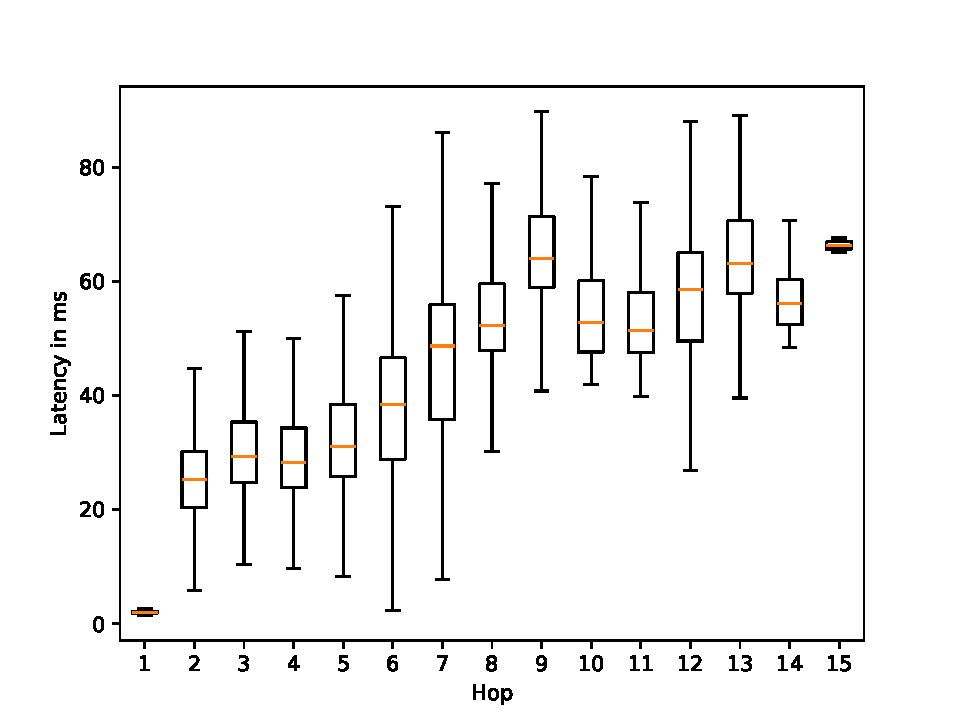
\includegraphics[width=\linewidth]{chapters/4-results/traceroute/img/latency-per-hop-ES.pdf}
		\caption{Spain}
	\end{subfigure}
	\begin{subfigure}[b]{0.48\linewidth}
		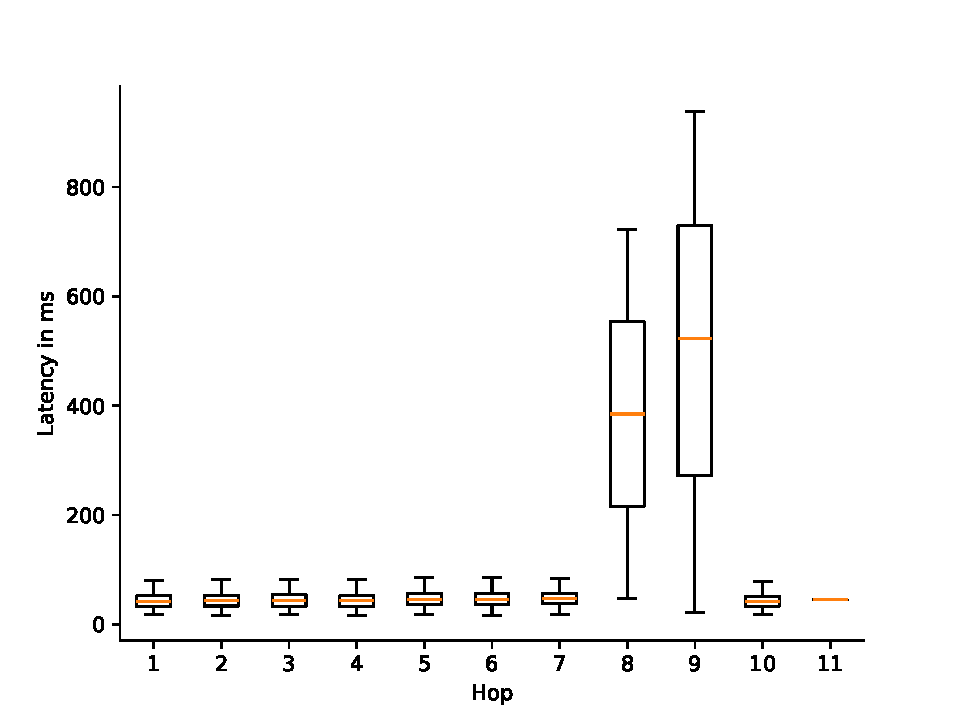
\includegraphics[width=\linewidth]{chapters/4-results/traceroute/img/latency-per-hop-CZ.pdf}
		\caption{Czech Republic}
	\end{subfigure}
	\begin{subfigure}[b]{0.48\linewidth}
		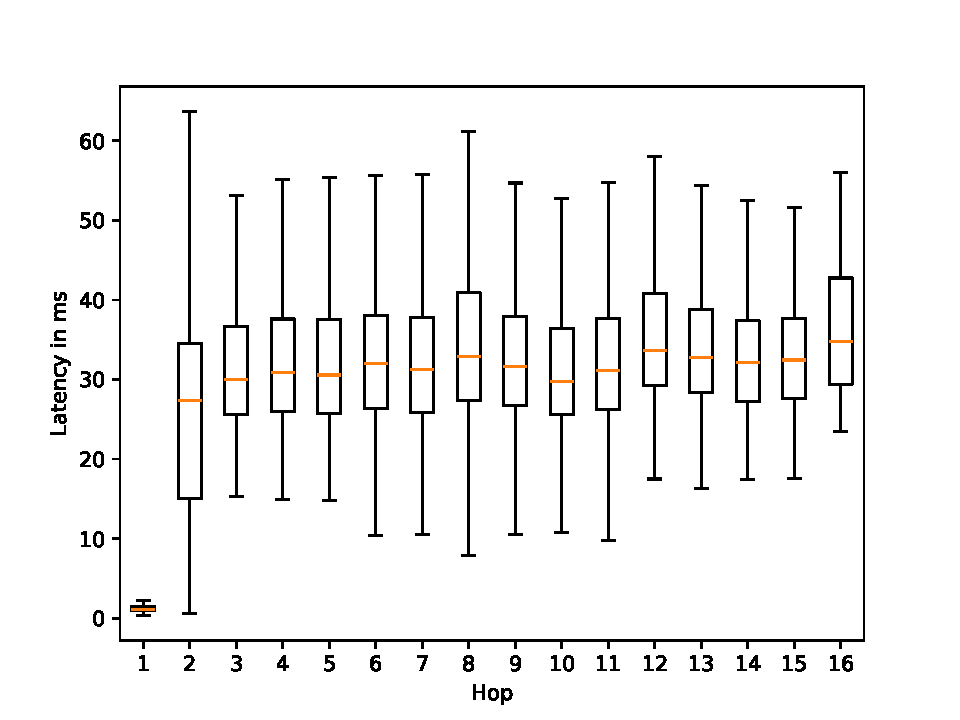
\includegraphics[width=\linewidth]{chapters/4-results/traceroute/img/latency-per-hop-GB.pdf}
		\caption{United Kingdom}
	\end{subfigure}
	\caption{Average Latency per Hop}
	\label{fig:latency-change-per-hop-appendix}
\end{figure}




